\documentclass{thesis-ekf}
\usepackage[T1]{fontenc}
\usepackage[english]{babel}


\usepackage{amsthm, url, array, float, graphicx, listings, xcolor, mathtools}

\newtheorem{theorem}{Theorem}[chapter]
\theoremstyle{definition}
\newtheorem{definition}[theorem]{Definition}

\theoremstyle{remark}
\newtheorem{remark}[theorem]{Remark}

\definecolor{custompurple}{RGB}{170,60,170}
\renewcommand{\lstlistingname}{Code Extract}
\lstset{
	language=Python,
	basicstyle=\color{white}\ttfamily\small,   % Set text color to white
	numbers=left,
	numberstyle=\tiny,
	numbersep=5pt,
	backgroundcolor=\color{black!80},   % Set background color to black
	commentstyle=\color{black!50},    
	keywordstyle=[1]\color{orange},    % Set keyword color to orange
	keywordstyle=[2]\color{custompurple},    % Set secondary keyword color to purple
	stringstyle=\color{green!75!black},       % Set string color to green
	breaklines=true,
	showstringspaces=false,
	frame=tb,
	framexleftmargin=5mm,
	rulecolor=\color{white},     % Set frame color to white
	xleftmargin=5mm,             
	xrightmargin=0mm,              
	morekeywords=[1]{if,else,for,while,import,from,class,def,return,try,except,finally,raise,global,nonlocal,lambda,assert,with,yield,async,await},
	morekeywords=[2]{self,\_\_init\_\_},   % Add more keywords (escape underscores)
}


\institute{Institute of Mathematics and Informatics}
\title{Web Scraping and Monte Carlo Simulations for Analytical Forecasting}
\author{Lorand Heidrich\\ Computer Science BSc}
\supervisor{Adam Kovacs\\ Teaching Assistant}
\city{Eger}
\date{2024}

\begin{document}

\maketitle


\clearpage
\section*{Acknowledgments}
\thispagestyle{empty} 
I would like to express my gratitude to Dr.~Eric Grono and Mr.~Garrett Weinzierl for their mentorship and support throughout my journey into the domain of Monte Carlo simulation and analytical forecasting. Their expertise, patience, and guidance have not only paved the way for new avenues of exploration but have also instilled within me an appreciation for the intersection of computer science and predictive modeling.

Their influence has played an instrumental role in shaping my academic and professional trajectory. I am indebted to them for their impact on my endeavors.

Thank you both for your generosity in sharing your time and knowledge, and your patience in addressing my myriad of questions throughout my studies. 


\tableofcontents


\chapter{Introduction}
In today’s world, data has become of paramount importance, profoundly influencing our lives and shaping decision making processes. The acquisition, processing, and interpretation of data is fundamental across multiple domains. \cite{Mondaut} Recognized as the cornerstone of contemporary insights, data serves as the basis of deriving valuable insights, and making informed projections, thereby guiding strategic planning and allowing for suitable preparation in the face of uncertainty. However, utilizing the full potential of acquired information effectively in a complex, multi-variable dynamic environment can be a challenging task \cite{Kornwitz}.

This thesis approaches data collection and forecasting from a sports analytical perspective, aiming to derive statistical insights and formulate projections regarding future performance. It endeavors to utilize a combination of web scarping techniques \cite{Khder} and Monte Carlo simulation \cite{Aderibigbe} for analytical forecasting. Through the integration of these techniques, this research aims to explore a comprehensive methodology for data acquisition and predictive modeling.

\section{Contextual Background}
The National Basketball Association (NBA) \cite{NBA} is well known for its worldwide prominence and dedicated fan base. Its enduring popularity has resulted in a multitude of analytical data relating to historic games. This abundance of statistical data, along with a widespread general awareness of the sport and my personal enthusiasm for it, positions historic NBA games an ideal domain for exploring predictive modeling based on data obtained through web scraping.

\section{Motivation}
The incentive for this research is derived from a keen interest in the technical intricacies of web scraping and probabilistic elegance of Monte Carlo simulations. The application of these techniques transcends the domain of sports analytics, with uses in finance \cite{McLeish}, physics \cite{Aderibigbe}, and beyond \cite{Steffen}.

\section{Objectives}
The primary objective of this thesis is two-fold. Initially, to employ web scarping techniques to gather comprehensive historical NBA game data from the early 1990s. Subsequently, to utilize said data to simulate a general probabilistic outcome for selected historic NBA games.

Specifically, the research aims to:
\begin{itemize}
\item Develop a multi-approach web scraping pipeline to gather comprehensive historical data for a given NBA season and team.
\item Manage and store the acquired data.
\item Implement a multi-epoch Monte Carlo simulation to model potential game outcomes based on the attained data through modeling offensive possessions.
\item Evaluate the predictive accuracy and reliability of the proposed methodology through empirical testing and validation against actual historic game results.
\end{itemize}
Through these objectives, this thesis undertakes to promote a deeper understanding of web scraping and predictive modeling within sports analytical forecasting.


\chapter{Methodology}
\section{Web Scraping Techniques}
\section{Monte Carlo Simulation}




\chapter{Requirements}

\section{Requirements List}
The system shall be constructed to uniquely fulfill both the requirements of a computer science thesis, and the domain of data acquisition and simulation based projections. It should therefore result in an intuitive end-user experience, leveraging the web scraping and Monte Carlo simulation methodologies explored in this thesis.

The client interface should allow users to interact with the business logic\footnote{The term refers to the collection of algorithms responsible for allocating and processing data through communication with the database in order to serve the user interface, while maintaining its independence from both. For further information, please see \cite{Booch}.}, thereby accessing the database through built-in functions. It should also allow for the utilization of web scraping and Monte Carlo methodologies. The Use Case diagram depicted below outlines the basic functionality described by the Functional - (see table {\ref{table-funct-req}}), Non-Functional - (see table {\ref{table-non-funct-req}}), and Platform Requirements (see table {\ref{table-platform-req}}) outlined in this chapter.

\begin{figure}[th!]
	\centering
	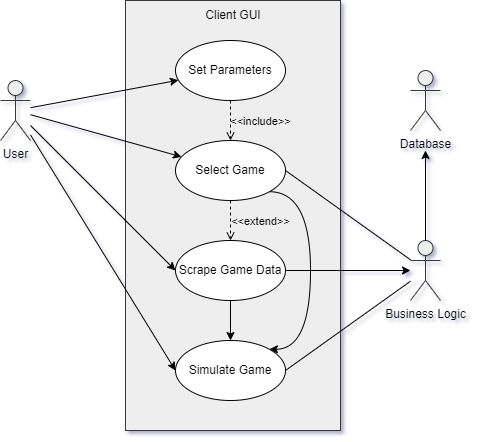
\includegraphics[width=7cm]{img/usecase}
	\caption{Use Case Diagram}
	\label{img-usecase}
\end{figure}


\subsection{Functional Requirements}
\begin{table}[H]
	\centering
	\begin{tabular}{|c|c|>{\raggedright\arraybackslash}p{10cm}|}
		\hline
		\textbf{ID} & \textbf{Name} & \textbf{Description} \\ 
		\hline
		R1	& Database & The system must allow users to select either the default database or utilize their own, based on a URI connection string. \\ 
		\hline
		R2	& Game Parameters & It should provide users with a method to set the season, home- and away team. \\ 
		\hline
		R3	& Epochs & The system must enable users to specify the number of epochs for the Monte Carlo simulation. \\ 
		\hline
		R4	& Game Data & Historic game data should be displayed based on these settings for user review. \\ 
		\hline
		R5	& Select Game & Users must be able to select an exact game to simulate from the displayed list of historic games. \\ 
		\hline
		R6	& Missing Game & The system must recognize if the selected historic game is not in the database. \\ 
		\hline
		R7	& Scrape Method & It should provide users with options for scraping the missing data trough different web scraping methods. \\ 
		\hline
		R8	& Proxies & Scraping options should include the ability to use proxies. \\ 
		\hline
		R9	& Proxy List & Users should have the ability to utilize their own proxy lists. \\ 
		\hline
		R10	& Forced Scrape & The system must allow users the option to scrape game data even when it is deemed unnecessary by the algorithm. \\ 
		\hline
		R11	& Validation & The system must ensure that data is not duplicated in the database. \\ 
		\hline
		R12	& Simulation & The system must execute Monte Carlo simulations based on the selected game parameters. \\ 
		\hline
		R13	& Graphs & It should visualize simulation results with graphs, including a probability density graph and a violin graph. \\ 
		\hline
		R14	& Metrics & The system must return basic metrics such as the number of wins for each team and the mode of scores. \\ 
		\hline
		R15	& Comparison & Users should be able to compare simulation results with original game data. \\ 
		\hline
	\end{tabular}
	\caption{List of Functional Requirements}
	\label{table-funct-req}
\end{table}

\subsection{Non-Functional Requirements}
\begin{table}[H]
	\centering
	\begin{tabular}{|c|c|>{\raggedright\arraybackslash}p{10cm}|}
		\hline
		\textbf{ID} & \textbf{Name} & \textbf{Description} \\
		\hline
		NR1 & Anonymity & The system must take steps to attempt anonymity throughout the web scraping process. \\
		\hline
		NR2 & Validation & It should validate user input parameters, throwing errors when incorrectly set. \\
		\hline
		NR3 & Errors & Users should be notified of errors during the application's operation. \\
		\hline
		NR4 & Logging & It must utilize a logging system to allow for easier debugging. \\
		\hline
		NR5 & Intuitive & The system must have an easy-to-use and intuitive interface. \\
		\hline
		NR6 & Requests & The client side of the system must communicate with the server-side logic using HTTP to attain services as a responses. \\
		\hline
		NR7 & SQL & The server-side logic should interact with the database using SQL queries. \\
		\hline
		NR8 & Database & The system must be able to utilize separate MySQL database servers. \\
		\hline
		NR9 & Testing & It should undergo thorough testing and validation to ensure accuracy, reliability, and robustness. \\
		\hline
		NR10 & Regulation & The system must comply with relevant legal and regulatory requirements. \\
		\hline
	\end{tabular}
	\caption{List of Non-Functional Requirements}
	\label{table-non-funct-req}
\end{table}

\subsection{Platform Requirements}
\begin{table}[H]
	\centering
	\begin{tabular}{|c|c|>{\raggedright\arraybackslash}p{10cm}|}
		\hline
		\textbf{ID} & \textbf{Component} & \textbf{Requirement} \\
		\hline
		PR1 & Client & The application should be compatible with Windows 10 (or later) operating systems. \\
		\hline
		PR2 & Client & The operating system is required to have .Net Framework 4.0.3 (or later). \\
		\hline
		PR3 & Host & Server environment must be capable of running a Python application with a Flask framework. \\
		\hline
		PR4 & Requirements & Back-end application requirements are available at: \url{https://github.com/lesheidrich/WebScraping_and_MCSim/blob/master/requirements.txt}. \\
		\hline
		PR5 & Database & The database server must be compatible with either XAMPP or MySQL. \\
		\hline
	\end{tabular}
	\caption{List of Platform Requirements}
	\label{table-platform-req}
\end{table}

\subsection{Use Cases}
\begin{itemize}
	\item \textbf{Game Selection}: The user selects parameters such as the desired season, home- and away team, to initialize game selection, then chooses the desired match from the returned table. 
	\item \textbf{Validation}: After accidentally setting a team to play against themselves, the user receives an error message alerting them of the mistake.
	\item \textbf{Scraping}: Following the game selection process, the system determines the game data is not in the database, then proceeds to utilize web scraping techniques to gather the data from online sources. 
	\item \textbf{Simulation}: A user parameterizes the number of epochs for the Monte Carlo simulation and initializes game selection. The system utilizes the acquired historical data to run simulations, generating probabilistic outcomes for the historic NBA game.
	\item \textbf{Comparison}: Users compare the results of the Monte Carlo simulation with the original game data, assessing the accuracy of the model. The system further provides probability density- and violin graphs to further facilitate result analysis.
	\item \textbf{Error Handling}: When the user tries to initialize game selection, the database is down. The host service returns an error, notifying the user of the access issue. The user escalates the error, and upon its resolution normal system operations resume.
\end{itemize}



\chapter{Architecture} \label{ch-architecture}
\section{Design Concepts}
At its core, the application relies heavily on a three principal layer \cite[p.~19]{Fowler} concept, commonly found in systems utilizing a database and presentation layer. Fowler refers to these as presentation logic, domain logic, and data source. The presentation logic facilitates user interaction with the system, the data source handles data transactions and houses application information, while the domain logic's algorithms are responsible for data modification and layer interaction. 

This is in line with the Gang-of-Four's \footnote{The Gang of Four \cite{GOF2} (GOF) are a group of four writers, all computer science professionals and entrepreneurs. Their literature and courses focus on professional development in the domain of computer science.} Model-View-Controller (MVC) \cite[p.~529]{GOF} design pattern. The View receives user-initiated interactions along with their parameters, and presents the application's data. It is capable of connecting directly to the model, while operating in conjunction with the Controller. The Controller interacts with both components as it processes their data and coordinates operations. The Model houses and manages the application data.

As discussed by Ahlan, A. R., Ahrnud, M. B., and Arshad, Y. \cite{Kulliyyah}, there have been several uses and variations of thin client applications since the 1970s. As a generalization, the \emph{view} in its capacity as the client receives application data and logic based services from a host system. This application adheres to the this concept quite strictly, with the client acting as an intermediary between the user and the host, taking use parameters and displaying host response results. The host service, operating as the back-end, encompasses the previously discussed Model, Controller and all other components of the application.

\section{Components}
Following the MVC design pattern's component structure, the application's presentation logic is allocated to the \emph{view} package. The database and simple business logic allowing for record management is stored in the \emph{model}. Acting as an intermediary between the two, the \emph{controller} package orchestrates the flow of information along with its processing. The \emph{webscraper} and \emph{simulator} packages also tie into the \emph{controller}, offering web scraping, and Monte Carlo simulation logic respectively, while further decoupling the application's components and allowing for better organization and maintainability through separation of concerns \footnote{Separation of concerns (SoC) is a software development design principle promoting segregation of source code elements by functionality in order to improve readability, organization and modification \cite{Reade}.}.

The application is organized in a manner, that all components embody system packages allowing improved readability and usability. The following subsections discuss each package's purpose and functionality.

\subsection{\emph{controller}}
\paragraph{Purpose:}
The package is responsible for processing component interaction, and serves as the core logic of the system.
\paragraph{Functionality:}
Serving as the system's host, the \emph{controller} is responsible for handling user prompts sent by the client in order to formulate an appropriate response. In order to fulfill this function it utilizes its connection to each component of the application, accessing their functionality as needed.

One of its responsibilities is accumulating data through the application of various web scraping methods, which are stored for future use. It's web scraper control functionality enables it to utilize the \emph{webscraper} package to appropriate preset website data into memory, then reallocate it to the database using a combination of its own control processes along with the business logic of the \emph{model} package. The web scraping sequence diagram illustrates the process (see {\ref{img-scraping-sequence}}).

When running a simulation for a parameterized game, the \emph{controller} restructures relevant data for the selected historic games from the \emph{model} into player, roster, and team objects usable by the \emph{simulator}. The simulator returns the results to the host, which are forwarded back to the client. The Monte Carlo simulation sequence diagram shows further details (see {\ref{img-monte-carlo-sequence}}).
\paragraph{Interaction:}
In its capacity as the main communications hub of the application, the \emph{controller} interacts with every component in the system. The package's component diagram provides a high level overview of basic component interaction (see{\ref{img-controller-component}}).
\begin{figure}[th!]
	\centering
	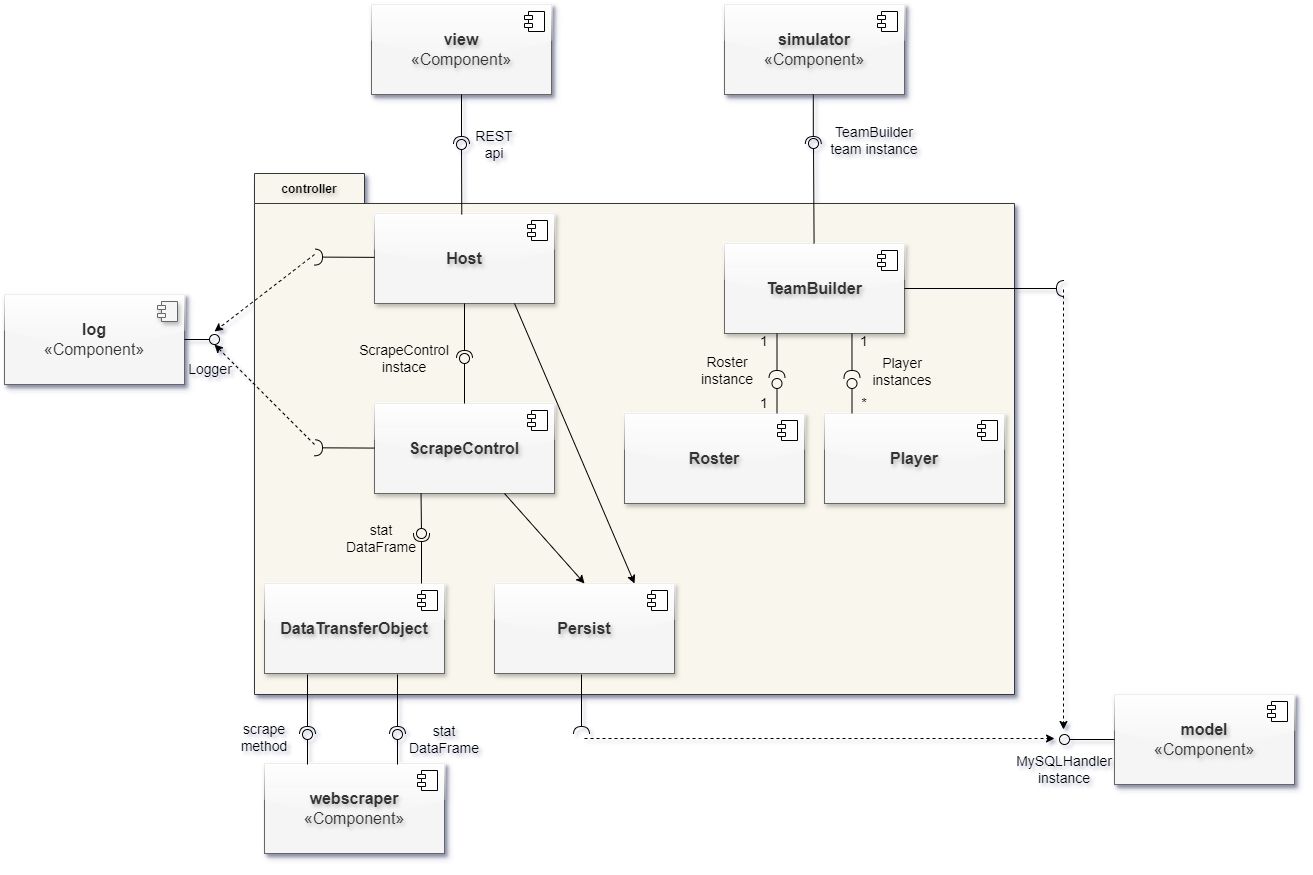
\includegraphics[width=1\linewidth]{img/component/component_controller}
	\caption{\emph{controller} UML Component Diagram}
	\label{img-controller-component}
\end{figure}

\subsection{\emph{log}}
\paragraph{Purpose:}
The component provides logging functionality for back-end operations.
\paragraph{Functionality:}
The \emph{log} package contains logic allowing components to access system logs to document runtime errors and operations, useful for debugging potential issues. Log management functionality is also provided by the package, ensuring proper settings, size limitations and functionality.
\paragraph{Interaction:}
The \emph{log} interacts with the \emph{controller} and \emph{webscraper} packages.

\subsection{\emph{model}}
\paragraph{Purpose:}
The package ensures successful data management services within the application, through the storage and manipulation of data records and structures. 
\paragraph{Functionality:}
The business logic enables system interaction with the database, encapsulating data access and administration services. Data security is enforced by minimizing vulnerabilities and prevents data corruption trough validation logic. The \emph{model} services the system through the \emph{controller} package's data manipulation and retrieval components.

The package also contains the NBA team enums \footnote{In their capacity as a distinct object type, enumerations (enums) offer value binding across a group of encapsulated constants tied together through enumeration. Each value can act as a key identifier during instantiation, making enums a powerful structure for housing validated data \cite{enum}.} employed by the back-end logic. These ensure data validation and encapsulate all occurrences of team names in the system and its dataset, streamlining their application throughout processes.
\paragraph{Interaction:}
The primary business logic elements of the \emph{model} communicate exclusively with the \emph{controller}, enhancing system modularity (see {\ref{img-controller-component}). Due to their earlier described functionality, NBA team enums are also widely employed throughout the \emph{simulation} package. 

\subsection{\emph{simulation}}
\paragraph{Purpose:}
The package's primary objective encompasses the repetitive simulation of a basketball game between selected teams at a specific point in time, with the end goal of returning the outcomes as graphical representations, comparable with the original historic game's outcome.
\paragraph{Functionality:}
The core functionality of the application revolves around implementing Monte Carlo simulations over a preset range of epochs to determine the probabilistic outcome of a historic NBA game. 

The \emph{simulator} package receives the relevant compiled data from the \emph{controller}, initializing the creation of the simulation. Upon successful completion of the simulation, probability density and violin graphs are returned to the \emph{controller} along with minimal game statistic like total win percentage and mode of scores reached per team. A detailed description of the process is illustrated in the Monte Carlo simulation's sequence diagram (see {\ref{img-monte-carlo-sequence}}).
\paragraph{Interaction:}
The \emph{simulator} relies on the \emph{model}'s NBA team enum during operation, along with the \emph{controller} for providing the necessary historic game data for simulation's successful operations. It further communicates with the \emph{controller} in its capacity as the host. The \emph{simulation} component diagram offers an overview of component interaction (see \ref{img-simulation-component}).
\begin{figure}[th!]
	\centering
	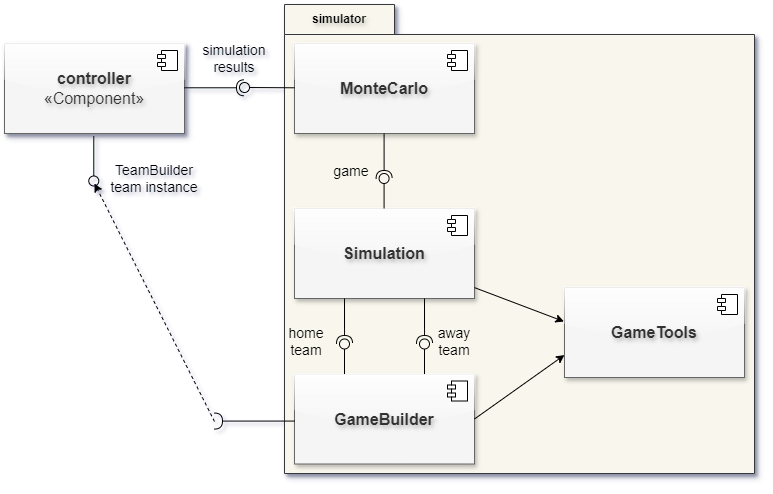
\includegraphics[width=0.7\linewidth]{img/component/component_simulation}
	\caption{\emph{simulation} UML Component Diagram}
	\label{img-simulation-component}
\end{figure}
\begin{figure}[th!]
	\centering
	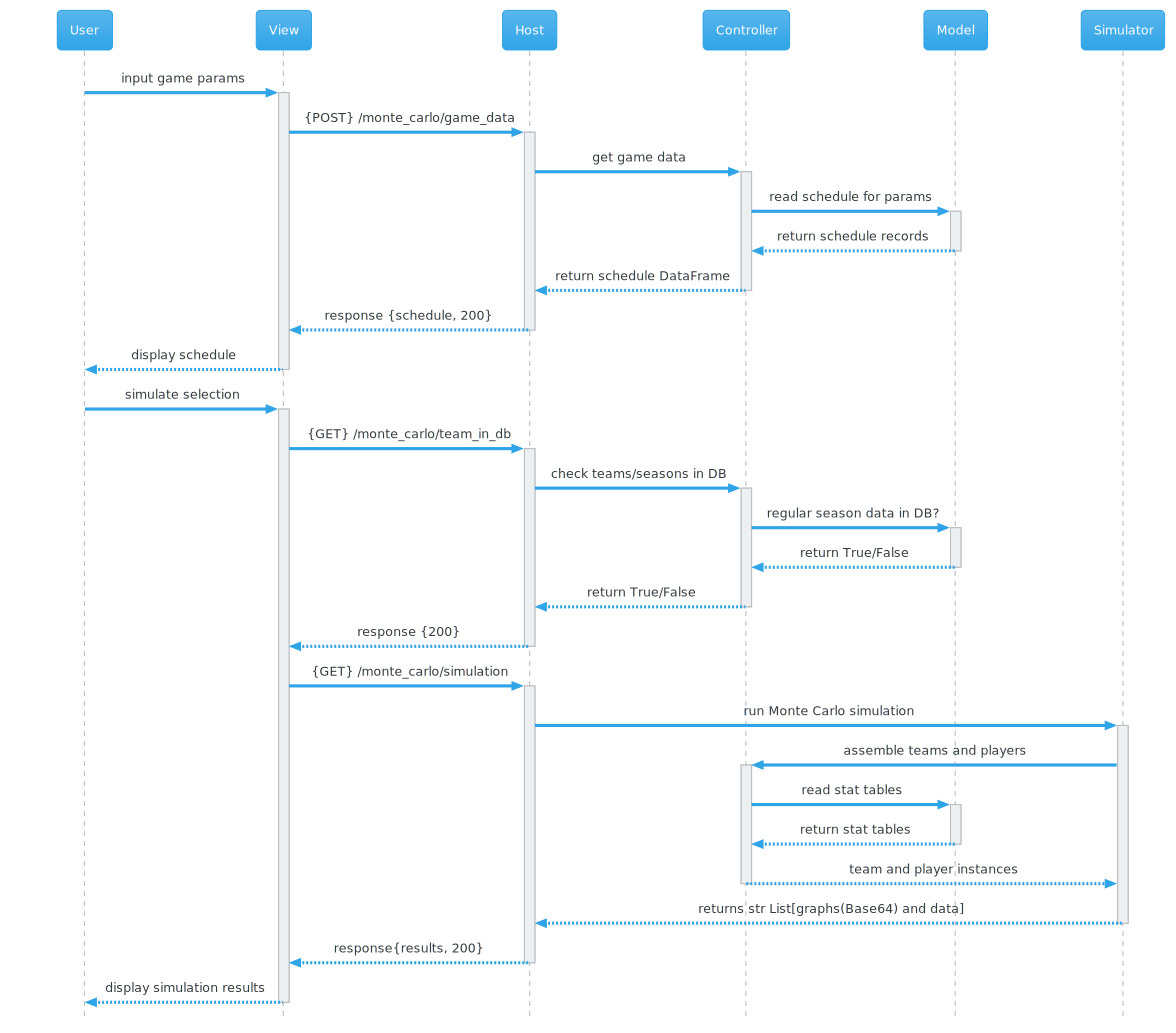
\includegraphics[width=1\linewidth]{img/sequence/monte_carlo/monte_carlo_sequence_cerulean}
	\caption{Monte Carlo Simulation UML Sequence Diagram}
	\label{img-monte-carlo-sequence}
\end{figure}


\subsection{\emph{test}}
\paragraph{Purpose:}
The component is responsible for providing comprehensive back-end testing services.
\paragraph{Functionality:}
The test package constitutes a wide spectrum of tests focusing on the back-end of the system. It provides full-scale uni tests organized by module. Integration testing and linting is also included. The Testing and Validation chapter (see \ref{ch-testing}) contains a detailed breakdown of the package's functionality and implementation.
\paragraph{Interaction:}
Each unit test interacts with their respective components on the back-end. Integration tests interact with multiple packages following their functionality, in their attempt to check full system compatibility.

\subsection{\emph{view}}
\paragraph{Purpose:}
To allow for user interaction with the system through communication with the host along with its application logic and data.
\paragraph{Functionality:}
The view package operates as a thin client, taking user input through a graphic user interface (GUI) \cite{Wiki-GUI}. User data is cached on the client side for the sake of user convenience, decreasing the input required to achieve functionality. Host responses, along with operational errors are displayed for user viewing. Errors are not logged on the client side of the application.
\paragraph{Interaction:}
The component interacts with the user and the host module of the \emph{controller} package.

\subsection{\emph{webscraper}}
\paragraph{Purpose:}
The package completes data gathering services from the amalgamation of preset websites and parameters representing selected NBA games, in order to supply historic statistical game data for the application.
\paragraph{Functionality:}
The acquisition process extracts data from a combination of preset URLs, set to match parameterized game data originating from the user. It includes functionality to interact with each URL in a manner defined by the user's chosen scraping method. Collected information is preprocessed and transformed before being committed to memory in a preset reusable format, easily accessed by the \emph{controller} as it looks to the \emph{webscraper} to acquire new information. Web scraping requests are generally not repeated, as the system is built to house already accessed data, thereby minimizing dependency on online sources to bare necessity. The component's sequence diagram (see \ref{img-scraping-sequence}) illustrates the process during runtime.
\paragraph{Interaction:}
The \emph{webscraper} package primarily communicates with the \emph{controller} in order to receive data acquisition requests and parameters. Its preprocessed results are also returned to the \emph{controller}. The package's component diagram (see \ref{img-webscraper-component}) illustrates the \emph{webscraper}'s interactions. Logging is utilized throughout the process.
\begin{figure}[th!]
	\centering
	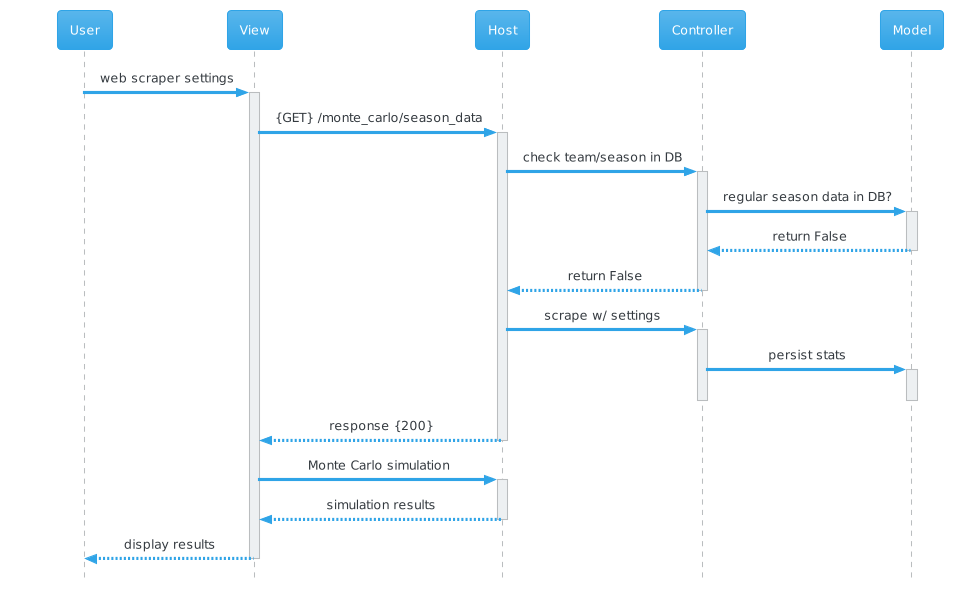
\includegraphics[width=0.9\linewidth]{img/sequence/scraping/scraping_caerilian}
	\caption{Web Scraping UML Sequence Diagram}
	\label{img-scraping-sequence}
\end{figure}
\begin{figure}[th!]
	\centering
	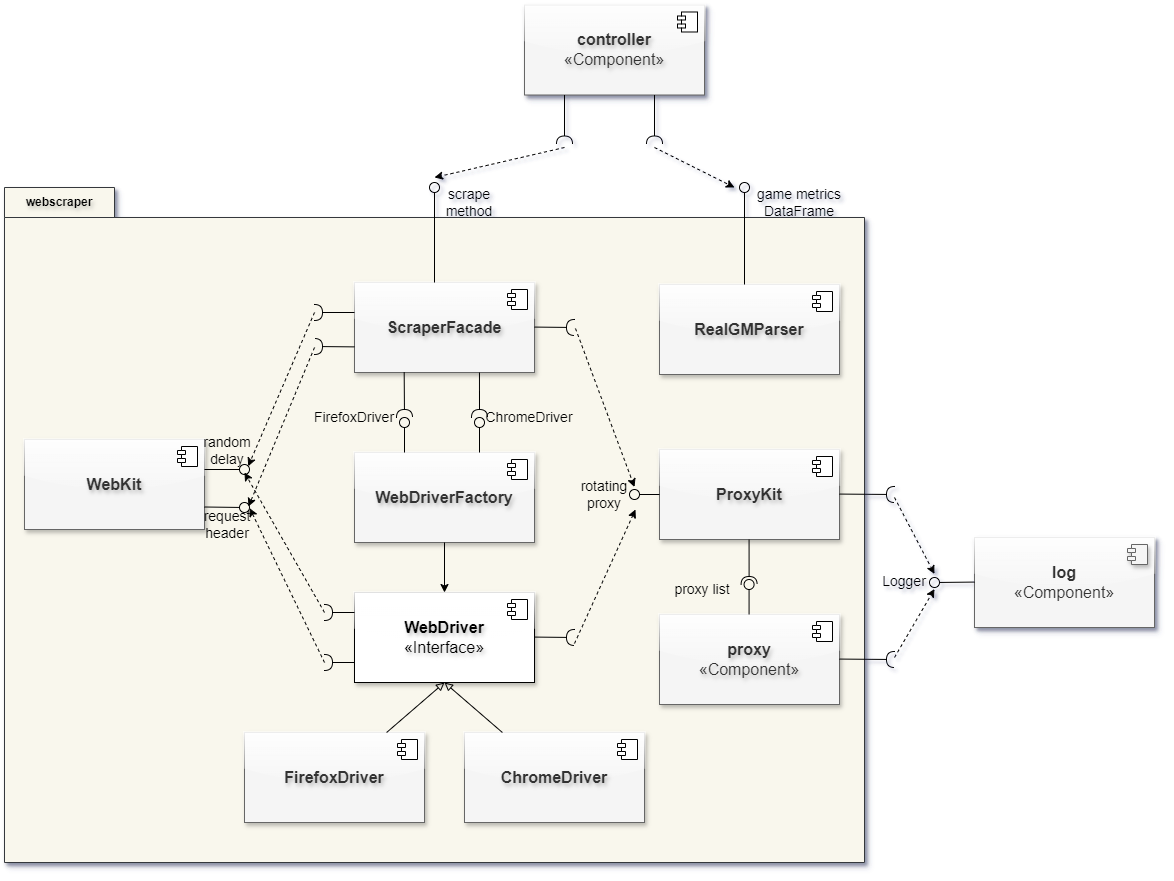
\includegraphics[width=0.7\linewidth]{img/component/component_webscraper}
	\caption{\emph{webscraper} UML Component Diagram}
	\label{img-webscraper-component}
\end{figure}

\section{Database Architecture}
The database consists of two main table types: utility tables and tables containing relevant game metrics. The utility tables are static, and assist in the application's game related logic, while metrics tables house data scraped from the web to be utilized in the simulation process. 

\subsection{Utility Tables} 
\paragraph{\emph{in\_playoffs}:} This is a boolean table pairing each NBA team (columns) to a season of game-play (records). Teams that made the playoffs receive a 1, while teams that failed to make the playoffs in the given season are left NULL.

\paragraph{\emph{schedule}:} The table houses historic NBA game dates and outcomes, along with the game type (regular or playoff game). Records range from the commencement of the 1990-1991 season until the end of the 2022-2023.

\subsection{Metrics Tables}
There are three types of metrics tables:
\begin{itemize}
	\item \textbf{Individual game tables} contain game data for each individual NBA game. Multiple player records are available for each date, with stats portraying the players performance for the single game. Separate tables exist for regular season and playoff games.
	
	\item \textbf{Player tables} are unique to each player of each team. They represent the player's averages for the given season. Due to the differences in performance, separate tables exist for home and away games, but also for regular season and playoff games, making a total of four player tables.
	
	\item \textbf{Team tables} house averages pertaining to the each team's performance in the given season, therefore each team is unique to each season. Once again, due to the high fluctuation between regular season and playoff metrics, tables are separated into these two categories.
\end{itemize}
To ensure all information remains unique, yet no new data is erroneously deemed as a duplicate, all cells of a record are expected to be unique in each table. This constraint ensures data validation, as a player will not be able to appear twice in relation to a game date with all the same metrics, or in the same season. Teams undergo the same validation process, being unique for each season.

Table metrics are presented in more detail during the \ref{sec-simulation} \emph{simulation} and \ref{sec-webscraper} \emph{webscraper} sections of the Implementation chapter.

\section{Technologies and Frameworks}

\subsection{.NET}
The .NET framework was built by Microsoft for developing Windows-based applications. Today, with the integration of cross-platform and open source frameworks, the .NET Core supports multiple operating systems and is also open source. It supports multiple programming languages, including C\#. \cite{.net}

The view component of the application is based on the .Net framework and written in C\#, due to its ability to model a range of services. It's WinForms (see \ref{winform}) framework and RestSharp package allow for fast and secure development, as well as a seamless user exprience.

\subsection{Beautiful Soup 4}
Beautiful Soup \cite{bs4} is a popular python package, designed to extracts data from HTML 
  \footnote{HyperText Markup Language (HTML) is a markup language used to house online content and set its layout, thereby creating the basic structure of web pages \cite{mdn-html}.}
and XML 
  \footnote{Extensible Markup Language (XML) is a markup language for data transfer and storage.
  Rather than offer preset tags, users can organize content subjectively through the application of a key value pair data structure \cite{mdn-xml}.}
documents sourced from the web. By leveraging attributes unique to the selected markup language, it facilitates tag and text content based parsing in order to precisely identify and extract the desired data. Developed for web scarping purposes, it is often used alongside packages responsible for making content requests to websites. 

This was also the case in this project. Beautiful Soup was a great asset during the allocation and extraction of acquired web contents, which could then be passed on for further formatting and storage.

\subsection{Fake User Agent}
Throughout the extraction of data from websites it is crucial to consider the exchange of information between the client making the request, and the website's host server responding to the request. During this process, the host receives client information in the header, allowing it to discern information about the requesting client, like its operating system and browser type (see subsection \ref{sub-http} for information on HTTP requests and their headers).

Operations requiring repeated content requests to a single host, such as web scraping, can therefore be identified as outside the scope of regular usage requirements provided by the website. This in turn may lead to limitations of service, disrupting web scraping-based system operations.

Fake user agent applications are designed to solve this problem. Python's \emph{fake-useragent} library allows for the creation of random user agent headers, which can be assigned to requests \cite{fake-useragent}. Users have the option to select from a wide range of preset options, which can also be filtered to only mimic specific browser technologies and operating systems. While this method only changes a portion of the request data, when used alongside other methodologies promoting anonymity, it can prove to be a powerful tool.

The package was employed in the project for this ability to generate random user agents at runtime, thereby contributing to the application's anonymity while web scraping.

\subsection{Flask}
Flask is a Python based web framework created to facilitate the development of web applications. The framework is known for its versatility, and aims to provide a minimalistic and flexible approach in comparison with other web application frameworks \cite{docs-flask}. 

Developers can choose their server platforms and environments, as Flask's WSGI (Web Server Gateway Interface) specifications enable it to integrate with a multitude of web servers, such as Apache and Nginx \cite{flask}.

Flask also contains a built-in development server, which provides application testing and debugging features. It also supports other extensions and libraries, granting integration capabilities to developers to handle session management or database connectivity. The framework focuses on the provision of necessary tools instead of enforcing constraints, thereby making Flask a popular web framework \cite{flask}.

The framework was employed in the application due in part to its ease-of-use and flexibility. The host required a lightweight solution compatible with Python. A robust strict framework such as Django would have hindered the timely development of the project, and Flask's accessibility made it a great candidate.   

\subsection{HTTP} \label{sub-http}
Hypertext Transfer Protocol (HTTP) is a method of communication employed to facilitate data exchange between servers hosting web-based resources, and clients such as web browsers or web-applications \cite{mdn-http}.

HTTP is unidirectional, operating on a request-response basis. When the client, such as a web browser requests services in the form of online content from a server, it does so through an HTTP request. The server processes the request, and sends an appropriate HTTP response. Data can be transmitted in multiple formats. Common examples include JSON 
 \footnote{JavaScript Object Notation (JSON) is a popular lightweigth data structure which utilizes key-value pair functionality. Due to it's simplicity and compatibility with many programming languages it is a common choice for online information exchange \cite{mdn-json}.}
, HTML, and XML \cite{wiki-http}.

The client's request contains information such as the request line, message body, and headers \cite{req-head}. The request line contains the destination resource, the message body stores parameters used by request methods, and the headers contain information about the client's choice of operating system and web browser. The response is comprised of a status code, headers and message body, which houses the requested data \cite{wiki-http}.

HTTP offers methods which can apply parameterized actions to the selected resource. Some examples include:
\begin{itemize}
	\item The GET method presents the specified resource. 
	\item POST submits data parameters to the server which are required for further functionality.
	\item PUT is used to update a selected resource on the server.
	\item The DELETE method removes the parameterized resource from the server.
\end{itemize}

Status codes are utilized to indicate the outcome of processes initiated by the client's HTTP request. They are categorized into groups, covering categories such as informational responses of success as well as errors. Some common examples of success codes include:
\begin{itemize}
	\item 200: The requested transaction was completed successfully and the requested content is returned.
	\item 204: The server processed the request, and is not returning any content.
	\item 400: A client error obstructed the server's attempt to complete the request.
	\item 404: The server does not contain the requested resource.
	\item 500: Indicates the occurrence of an internal server error, obstructing the fulfillment of the client request.
\end{itemize}

Due to security concerns, a more secure version of HTTP Secure (HTTPS) \cite{wiki-https} was created. It employs encryption mechanisms to ensure transaction security, thereby thwarting potential eavesdropping and tampering attempts. 

\subsection{Matplotlib}
Matplotlib is an extensive community-maintained Python library utilized in the creation of static, animated, and interactive visualizations \cite{matplotlib}. Matplotlib offers a wide range of functionalities, making it a versatile tool for data visualization tasks. It's Pyplot module allows for the creation of customizable and embeddable graphs and diagrams.

Ultimately the plotting capabilities of the package's Pyplot module led to its utilization in the system.

\subsection{MySQL}
MySQL is a free open source relational database management system (RDBMS). It is widely used due to it's speed, reliability and scalability. Structured Query Language (SQL) is utilized to communicate with the database for data management and user access modifications. \cite{wiki-mysql}

The decision to use MySQL as the application's database management system was reached due to several factors. The application required a relational model for easier storage of acquired statistical data, which in turn allowed easier processing upon extraction from the database. Its reliability and complementary open source nature, coupled with its widespread adoption and accessibility solidified the decision to utilize it in the application.

\subsection{Pandas}
The pandas library is an open source project developed for Python by Wes McKinney and Chang She during their time at  AQR Capital Management. The developers sought to attain the tabular functionality of DataFrames \footnote{DataFrames are two-dimensional tabular data structures in pandas, housing data accessible by rows and columns. Visually, DataFrames resemble spreadsheets, while structurally they key-value pair data structures. \cite{wiki-pd}}} in the R programming language for their flexibility and functionality in working with financial data. \cite{wiki-pd}

Pandas remains an open source library to this day, and has become very popular for its versatility and functionality in data analysis endeavors. It has been employed in this project due to this high level of tabular functionality and data accessibility, along with its efficiency in parsing tabular data into DataFrames.

\subsection{Python} \label{sub-python}
Python is a high level open source object-oriented programming language, with features such as dynamic typing, dynamic binding, and built in data structures. It is an interpreted language with a modular structure, and an easily readable syntax. \cite{python}

The programming language was utilized for the back-end due to its extensive complementary open source library. There availability of multiple web scraping packages, along with powerful data analytics libraries such as pandas or matplotlib allow for convenient and fast paced development.

\subsection{Requests}
The Python requests library is a simple package allowing for communication through HTTP requests. \cite{req} It is utilized in the application for making requests to specified websites in order to retrieve their HTML content in the response. Requests allows for parameterized customization of proxies, timeout settings, and request methods, many of which are utilized in the web scraping process. 

\subsection{REST API}
Representational State Transfer (REST) refers to a set of principles acting as guidelines in the development of APIs for web services. These stipulate the use of HTTP as a communication protocol, however data encoding is left up to the developer, with options including JSON, HTML, and XML. Requests should be independent, not relying on each-other's success. Caching of data is acceptable, along with the sending of executable code to the client where needed. REST further requires a standard method of sending data and a layered organizational approach. \cite{redhat-rest}

In the application, REST is utilized to facilitate communication between the client and host. HTTP requests are sent to the host in order to receive responses in the form of JSON.  

\subsection{RestSharp}
RestSharp is a tool utilized in .NET development, offering synchronous and asynchronous communication to remote resources using HTTP. It allows for easier managing of diverse request and response types while interacting with APIs by handling serialization and deserialization of message bodies to JSON and XML. \cite{restsharp}

The package is utilized on the client side of the application, due to these capabilities. Its GET and POST methods handle interactions with the host's API. Response JSONs are deserialized to access response content.

\subsection{Selenium}
Selenium is an open source test automation tool created for web applications. It enables developers to single out and interact with user interface (UI) elements thereby simulating user interaction. Selenium's WebDriver tool allows for the utilization of web browsers to interact with online sources, enabling programmatic clicking of buttons, mouse movements, and traversing web pages. Selenium supports multiple programming languages, including Python. \cite{selenium}

While driver instantiation already allows for the use of well known browsers, such as Mozilla's Firefox and Google's Chrome, the open source community has further contributed packages such as Undetected ChromeDriver. This Python library aims to provide the same driver functionality, while attempting to be less detectable by the host server. \cite{udc}

This project utilizes Python's Selenium package for web scraping purposes. Instantiating the driver allows for content retrieval in a less detectable, albeit slower manner.

\subsection{TestStack.White}
White is a test automation framework used to test Windows desktop applications. It is based on the .NET framework and does not require the use of scripting languages. Test code can be written in any .NET supported language. \cite{docs-white}

The framework is implemented in the project for UI automation testing purposes. The client's WinForms-based desktop application is tested for returning appropriate responses and basic functionality for quality assurance purposes.

\subsection{WinForms} \label{winform}
Windows Forms (WinForms) is a .NET graphical user interface (GUI) framework for building desktop applications. It provides developers with controls for dragging and dropping elements to rapidly create interactive user interfaces. \cite{winforms}

The application's client interface is built with WinForms in the C\# programming language. WinForms allowed for timely and precise development process, creating a visually appealing Windows desktop application.

\subsection{XAMPP}
Cross platform Apache MariaDB PHP Pearl (XAMPP) is a complementary open source web server solution stack meant for development environment utilization. Originally developed by Apache Friends, the application is widely used for testing and development purposes. It's available for multiple operating systems and makes the conversion process to a live server seamless, as it utilizes the same tech stack utilized by most production environments. \cite{wiki-xampp}

MariaDB, the open source database server used by XAMPP, is a fork of the the original MySQL. It was created with the intention that the project remain free and open source. \cite{mariaDB} As a fork of MySQL, it shares a high level of compatibility with it, and has been included in the project for this purpose. While XAMPP employs MariaDB, the project's business logic utilizes MySQL related code and Python libraries. This compatibility allows the application to access both MySQL servers and XAMPP's MariaDB-based service.

XAMPP is utilized as a development environment in the project, housing the application's built in database. It was chosen for its robust functionality and online user interface, which made testing during the creation and implementation of the model a more user-friendly experience. 


\chapter{Implementation}
In keeping with the structural approach of the Architecture chapter, the project's implementation is presented by package. Each section will delve deeper into the modular and functional breakdown of the project, along with their application. As other components require its presence, the \emph{model} package is introduced first, along with an introduction of the business logic.

\section{\emph{model}}
The \emph{model} package contains two classes: \emph{Teams}, and \emph{MySQLHandler}. They represent the business logic, responsible for encapsulation of the database's operations for data manipulation and contain the enum ensuring team names are handled appropriately throughout the application. As figure \ref{img-model-class}'s class diagram shows, the package mainly services the \emph{controller}, with the \emph{simulator} also utilizing team enums for smoother operations.
\begin{figure}[th!]
	\centering
	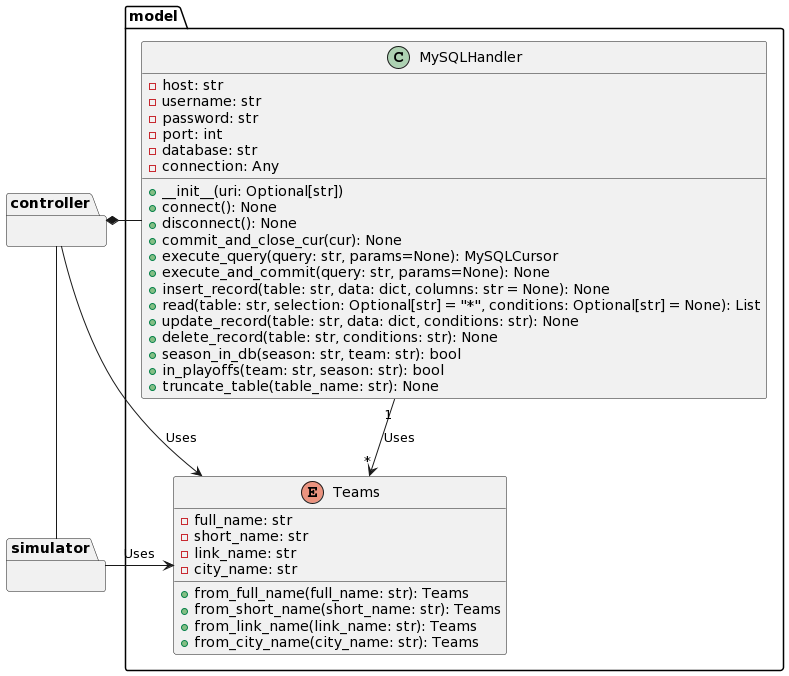
\includegraphics[width=0.8\linewidth]{img/class/model}
	\caption{\emph{model} UML Class Diagram}
	\label{img-model-class}
\end{figure}

\subsection{\emph{Teams} Enum}
The Teams enumeration represents each NBA team in the database in all forms of their use throughout the application. These are:
\begin{itemize}
	\item \textbf{Full Name}: represents both the city and team name (e.g.: Chicago Bulls).
	\item \textbf{Short Name}: short form of the team's city (e.g.: CHI).
	\item \textbf{Link Name}: both the city and team's name along with their unique id number as used in RealGM website URLs (e.g.: Chicago-Bulls/4).
	\item \textbf{City Name}: only the city the team plays for (e.g.: Chicago).
\end{itemize} 
The class contains logic to create enums from each of these name forms, along with the logic for displaying their converted values.

\subsection{\emph{MySQLHandler}}
The class facilitates communication with a MySQL or MariaDB database, initialized through the parameterized URL string. The connection string is parsed to allocate the correct sub-strings of the parameter to each class attribute (such as host, username, password, and port). Python's \emph{mysql.connector} library (see \cite{mysql.conn} for details) then proceeds to establish a connection to the database, allowing for use of the provided data management methods.

This initialization method allows the application to establish a connection at will with the user's database of choice. 

Data management functionality is customizable and secure, due to cursor parameterization with placeholders for dynamically inserting values into SQL queries. This decreases the likelihood of injection attacks, which would otherwise modify the code with malicious intent, or access unauthorized information \cite{injection-attack}.

Data modification proceeds through a query execution function, which initializes a cursor and attempts to execute the parameterized query string. Changes are rolled back upon encountering potential connection errors. Code Extract \ref{code-exec-query} illustrates the source code of the method. Upon successful completion of the operation, a separate function handles the commit to the database, and closes the cursor.
\lstinputlisting[caption=Cursor Execution of Query, label=code-exec-query]{code/exec-quer.pas}

While the client side of the application does not require update, delete, and truncate methods, the functionality has been included in the data access layer to enable comprehensive data management from the back-end.

\section{\emph{controller}}
The package is responsible for the implementation of three high level functionalities: the API host service, web scraping, and constructing \emph{TeamBuilder} NBA team instances for the simulator. Each of these controls manage a designated section of the back-end logic's operations. 

As discussed in the Architecture chapter (see \ref{ch-architecture}), the \emph{Host} amalgamates final operations of both web scraping -, and Monte Carlo simulation services. Web scraping operations are coordinated by the \emph{controller}'s \emph{ScrapeControl} class, while NBA team instantiation is handled by the \emph{TeamBuilder}. Team instances are provided for the \emph{simulator} package, which in turn services the \emph{Host}. The following sub-sections presents each functionality in detail.

\subsection{Host Service}
The \emph{host\_service.py} module houses the \emph{Host} class containing the Flask server handling requests pertaining to the functionality provided by the above described \emph{webscraper} and \emph{simulator} packages. Server instances handle these requests through the following endpoints and their respective class methods:
\begin{itemize}
	\item \textbf{/monte\_carlo/game\_data}: Its get\_game\_data() method reads the game schedule from the database based on the provided arguments, returning a JSON of the records to the client.
	
	\item \textbf{/monte\_carlo/team\_in\_db}: The get\_teams\_in\_db() method checks if the selected and previous season's data is present in the database for both teams, notifying the client of its findings.
	
	\item \textbf{/monte\_carlo/season\_data}: Its get\_season\_data() method initiates a scrape of missing game data. In case of failure, the method re-initiates the process for a second time, logging the attempt. The client is notified of the operation's success or failure via a REST response. In case of failure, the method removes records from the players table, thereby ensuring future checks will see it is still missing from the database.
	
	\item \textbf{/monte\_carlo/simulation}: The get\_monte\_carlo\_sim() initiates the parameterized Monte Carlo simulation, returning its results to the client. The JSON contains the probability density plot and violin plots as base64-encoded strings of the plot image files created by matplotlib. Basic game statistics are also included, such as modes of the score arrays, and win percentage. 
\end{itemize}

Flask instances are initialized with a timeout of 500 seconds, just over 8 min.~allowing adequate time for slightly longer simulations (see line 5 in Code Extract \ref{code-flask-init}). 

Utilizing matplotlib to create graphs during server runtime was challenging at first. When the server instance was running alongside the WinForms GUI, threading conflicts would randomly occur. This was because matplotlib's default back-end GUIs are not guaranteed to be thread-safe, therefore WinForms would occasionally attempt to utilize a resource already allocated to the plotting function. The solution was to set matplotlib to the Anti-Grain Geometry (Agg) plotting library (see line 3 in Code Extract \ref{code-flask-init}), which does not require the use of said resources. \cite{agg}

\lstinputlisting[caption=Flask Instance Initialization, label=code-flask-init]{code/flask-init.pas}


\subsection{Web Scraping}
The \emph{controller} package's web scraping functionality is encapsulated in two modules: \emph{control\_service} and \emph{dto\_service}. Each module's classes contribute specialized logic to the data gathering process. Together, the modules orchestrate the web scraping process, handle the transformation of data in memory, and manage persistence operations through interactions with the business logic. Figure \ref{img-controller-scrapecontrol-class} illustrates the package's class diagram pertaining to web scraping and data allocation logic.

\begin{figure}[th!]
	\centering
	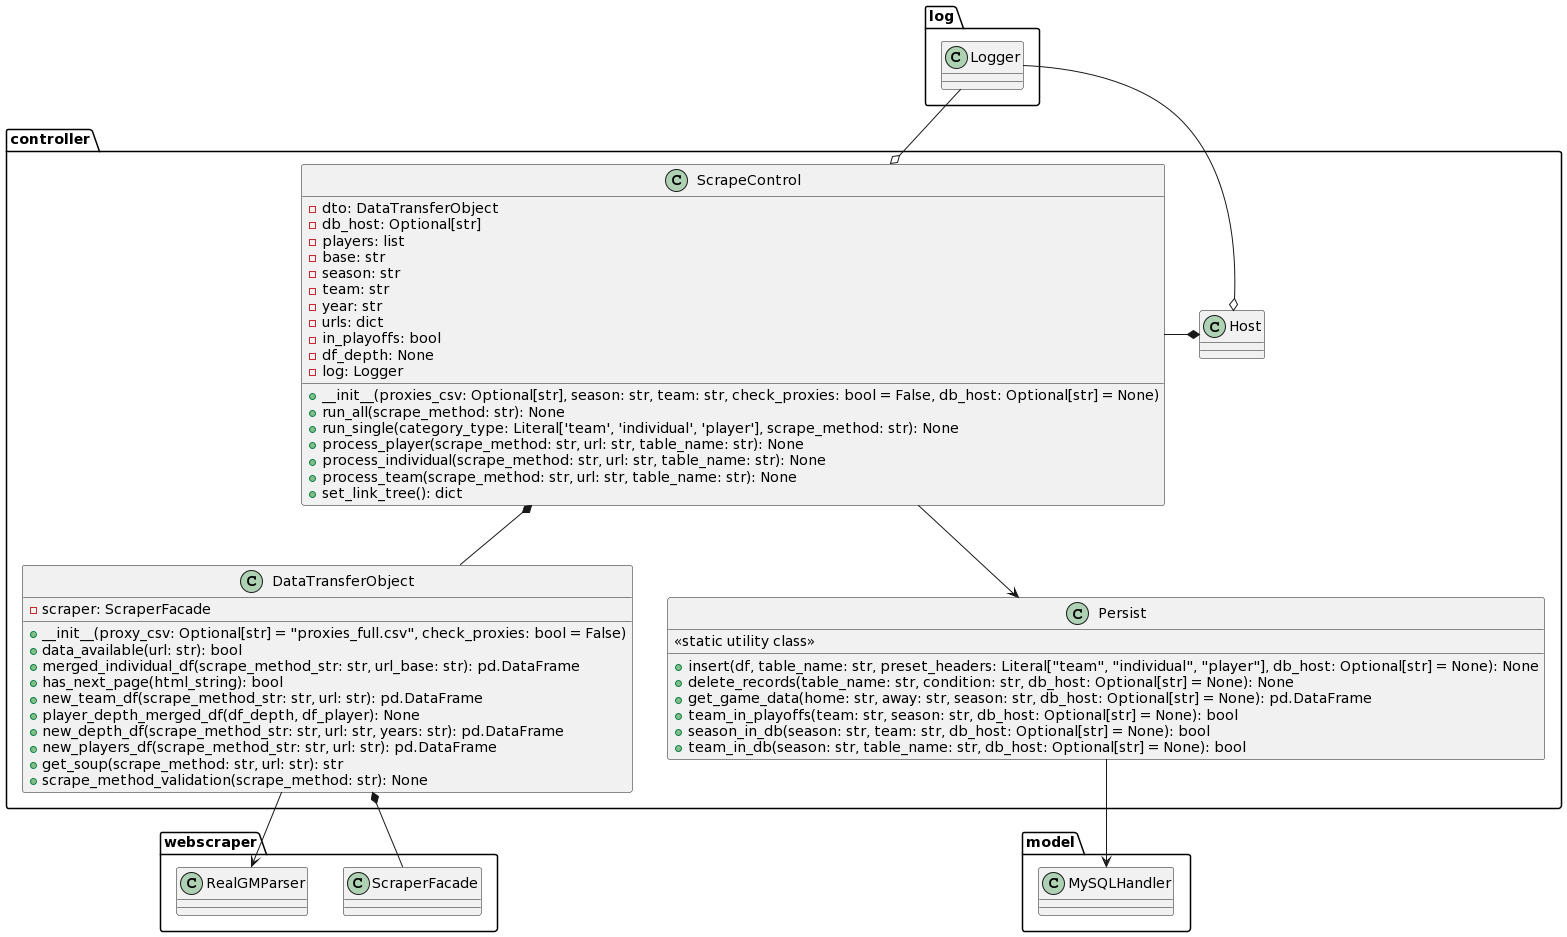
\includegraphics[width=1\linewidth]{img/class/controller_scrapecontrol}
	\caption{The \emph{controller}'s Web Scraping Services UML Class Diagram}
	\label{img-controller-scrapecontrol-class}
\end{figure}

\paragraph{The \emph{control\_service} module} houses the \emph{ScrapeControl} class. During initialization it:
\begin{itemize}
  \item Instantiates a \emph{DataTransferObject} (see section \ref{element-dto}) utilizing the specified proxy settings.
  
  \item Creates a dictionary of key-value pairs comprised of the parameterized URLs for each web page it intends to scrape data from.
  
  \item Assesses if the team is in the playoffs, storing a boolean from the result of the function call to \emph{Persist.team\_in\_playoffs}.
  
  \item Initializes a logger instance, and sets the necessary attributes for further operations.
\end{itemize}

The class is comprised of basic logic for scraping each table type, stored in the database: player, individual game, and team statistics. These are utilized by two main operating functions: \emph{run\_single} and \emph{run\_all}. This is because the application is designed to allow for simple use through a client interface, but also complex back-end use for a more detailed control of the process as required by analysts. The \emph{run\_all} method completes a full scrape for the chosen team and season, while the \emph{run\_single} method takes parameters allowing for further specification of the table type to acquire and populate (player, individual game, or team statistics).

The dictionary data structure housing the URLs allows for a controlled and detailed iteration, utilizing the assessment of the team's participation in playoffs for the given season set up during the instance's initialization. While iterating over the URLs, the appropriate scrape methods are utilized to attain raw HTML data as text, parse it to a Pandas DataFrame, and finally persist the data to the database. This functionality is further discussed in section \ref{sec-webscraper} titled \emph{webscraper}.

\paragraph{The \emph{dto\_service} module} contains the \emph{DataTransferObject}\label{element-dto} and \emph{Persist} classes. \emph{DataTransferObject} instances facilitate the retrieval of data through \emph{ScraperFacade} instances (see section \ref{sec-webscraper}). Users have the option to choose from a variety of scrape methods, with or without the utilization of proxies. The class further provides logic for handling data sourced from each pre-determined URL, flipping through pages where they are available, and storing them in Pandas DataFrames. 

Beyond utilizing services encapsulated by the \emph{webscraper} package, the class aims to alter and store data in memory for easier processing and better accessibility. Utilizing Pandas DataFrames as a data transfer object \footnote{Data transfer objects (DTO) facilitate data transfer between processes, where the only behavior allowed to the data structure is the storage of data \cite{dto-wiki}.} allows the class to compartmentalize data in structures that are easy to handle, debug, view and transfer to database tables.

With a collection of static utility methods, the \emph{Persist} class is responsible for handling data management operations within the application's database. Trough interaction with the \emph{MySQLHandler}'s business logic, it facilitates the insertion, deletion, and retrieval of data.


\subsection{Team Instantiation}
The \emph{dto\_sim} module contains three classes responsible for constructing NBA team instances: \emph{TeamBuilder}, \emph{Roster}, and \emph{Player}. \emph{TeamBuilder} instances create and house all data pertaining to teams participating in the match, with each team (home, and away) being a separate \emph{TeamBuilder} instance. Data is restructured and housed in \emph{Player} instances, which in turn are allocated to the appropriate position in the team's \emph{Roster}.

Once completed, team instances are utilized by the \emph{simulator} package's \emph{GameBuilder} class in the construction of individual game simulations. Figure \ref{img-controller-teambuilder-class} illustrates the class diagram relevant to the three classes responsible for team instantiation.

\begin{figure}[th!]
	\centering
	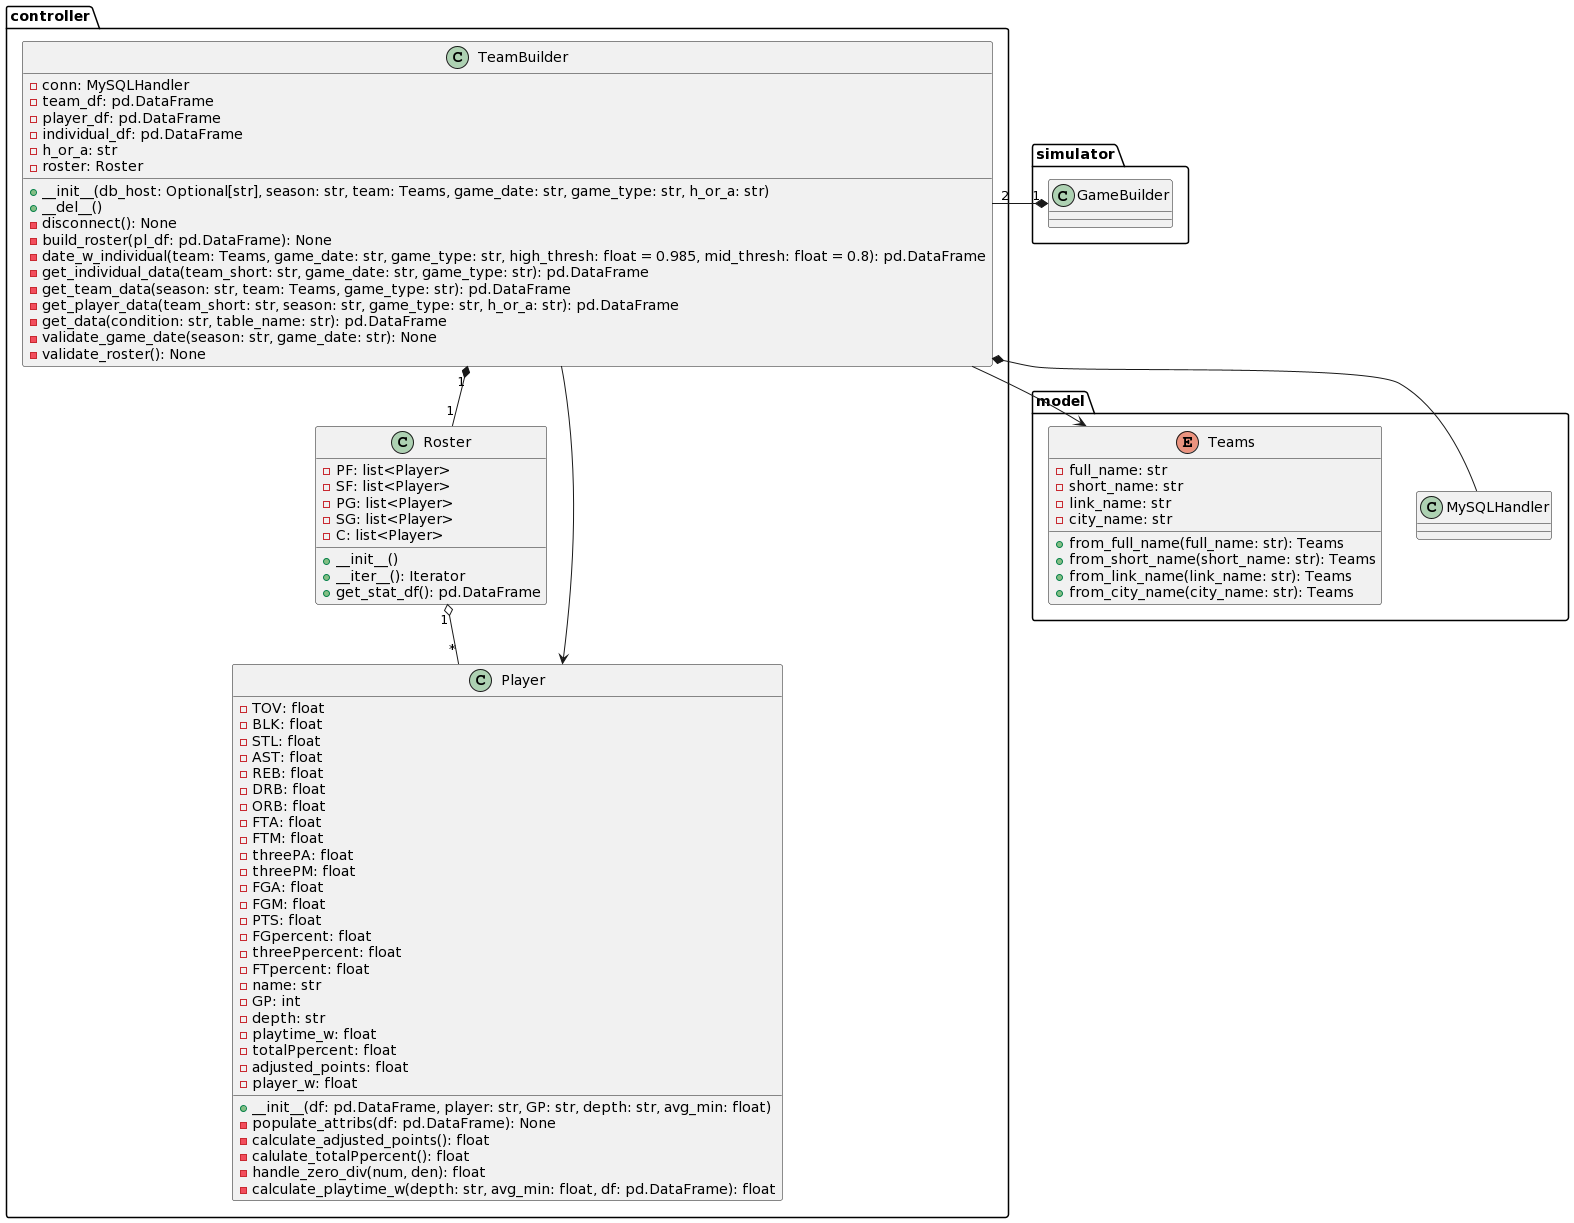
\includegraphics[width=1\linewidth]{img/class/controller_teambuild}
	\caption{The \emph{controller}'s TeamBuilder UML Class Diagram}
	\label{img-controller-teambuilder-class}
\end{figure}

\paragraph{\emph{Roster}} instances are only meant to function as iterable  containers. They are comprised of five empty lists upon initialization, each representing a playable position. These are:
\begin{itemize}
	\item PG - Point Guard: coordinates offense.
	\item SG - Shooting Guard: driving forward and scoring.
	\item PF - Power Forward: role is a mix between forward a center.
	\item SF - Small Forward: distance and inside scoring.
	\item C - Center: under basket game.
\end{itemize}
Each position list houses the \emph{Player} instances assigned to the respective position. The \emph{Roster} itself is also iterable.

\paragraph{\emph{Player}} objects store game statistics pertaining to the individual player. Even though I attempted to keep sports analytics to a minimum during the project, the list of attributes grew quite extensive. The majority of the statistics are derived from information already stored in the database. The exceptions are game metrics utilized as weights for decision making by the \emph{simulator}. Highlights of these metrics and the logic responsible for their calculation:

\begin{itemize}
	\item \textbf{adjusted\_points}: \\
	Adjusted points are an attempt to numerically categorize a player's true effectiveness via their affect on the team's offense, due to the player's direct contributions through points scored, rebounds, assists, etc. The are multiple approaches for this calculation. This project utilizes the model put forth by Jim Lackritz\footnote{Jim Lackritz is the co-founder of the Sports Business MBA program at San Diego State University's Fowler College \cite{SDSU}.} and Ira Horowitz\footnote{Ira Horowitz is an emeritus professor of statistics at the University of Florida \cite{SDSU}.}, available at the San Diego State University Fowler College Sports Business Program \cite{SDSU}.
	\begin{equation}
		\label{eq-adj-pts}
		\tag{Model 5.1: Lackritz's Adjusted Points Equation}
		\frac{3 \times \text{Total Points}}{4} + \frac{2.383 \times \text{Assists}}{4} + \frac{0.588 \times \text{Off. Rebounds}}{4} + \frac{0.530 \times \text{Steals}}{4}
	\end{equation}
		
	\item \textbf{player\_w}: \\
	A player's weight is the metric allowing the Monte Carlo simulation to make random weighted decisions about a players participation in the specified game. It is calculated by averaging the player's adjusted points percentage and playtime weight.
	
	\item \textbf{playtime\_w}:\\
	A players playtime weight is my arbitrary representation of a weight representing the player's probability to be on the court for any given possession. It utilizes the player's depth in the official roster for the season, and the player's average minutes played during the season divided by the number of minutes per basketball game (48). Second string players probability is then decreased to a quarter of its original value, why third string players are decreased even more, to 2\% of their original playtime. All other players are not considered during the simulation. 
	
	This is representative of a players playtime in a real life scenario, where third-string players will generally not see a lot of playtime unless the match itself is a statistical outlier. This can mean either injury, or the team performing so well or so poorly, that novice players can be introduced without detrimentally affecting the outcome of the match.
	
	This approach is a simplified representation of basketball analytics. More professional methods exist for calculating player utilization, however they are outside the scope of this project as it endeavors to approach the subject matter from a computer science perspective at the BSc level.
	
	\item \textbf{totalPpercent}: \\
	A player's total point percentage is calculated by averaging the percentage of their success rate from free throws, three pointers and field goals.

\end{itemize}


\paragraph{\emph{TeamBuilder}} instances are initialized, with the following operations:
\begin{itemize} 
	\item Validating the game date to ensure it falls within the required season.
	
	\item Creation of a Pandas DataFrame for each table category in the database:
	\begin{itemize}
		\item Individual games per player for specific game date.		
		\item Player table of seasonal averages.		
		\item Team table containing seasonal averages pertaining to the team.
	\end{itemize}
	
	\item The creation, population, and validation of a \emph{Roster} instance.
	
	\item Populating the necessary attributes for their functionality.	
\end{itemize}

It is important to note, that the three initialized DataFrames are filtered specifically to the parameterized data unique to each game. This decreases the demand on memory. Team statistics will therefore only contain one record for the instance's team in the season. Player statistics remain unchanged. The individual games table, however, is restructured, as player instance data is calculated from these.

The team's individual games table consists of one calendar year's data leading up to the game date. Code Extract \ref{code-get-ind-data} illustrates the source code responsible for compiling the DataFrame.
\lstinputlisting[caption=Initializing Individual Games DataFrame, label=code-get-ind-data]{code/get-ind-data.pas}
The DataFrame is then modified, repeating records pertaining to the last 2-3 games (those in the 98.5\% time span threshold of the game date) five times. Games falling within the 80\% threshold of the game date are repeated three times, while games in the more distant past only appear once in the re-constructed DataFrame. As all player data is reconstructed from stats in this DataFrame, more recent games will carry a greater weight in the player's performance. This is intended to represent the psychological affect an individual's recent performance has on their current output.

The \emph{build\_roster} method constructs \emph{Player} instances from the assembled DataFrames, populating them in their respective positions in the team's \emph{Roster}. This is done by iterating over each player in the players DataFrame. A boolean test ensures the player is assigned to a position (novice players that don't see playtime are not always assigned to positions). This is a preliminary filter to once again decrease the strain on memory. Second, the logic ensures the player is present in the individual games DataFrame. This ensures the player has seen playtime in the past 365 days. Players that do not meet this criteria are overlooked during the team construction process, as their chances of seeing playtime would be minuscule in reality as well. This further decreases demand on memory and computing time. All players who meet the requirements of the test logic are instantiated utilizing the individual games DataFrame filtered to the player's stats, and additional stats from the player DataFrame. Code Extract \ref{code-build-roster} illustrates the testing and appending functionality of the method.
\lstinputlisting[caption=Code Snippet of Roster Construction, label=code-build-roster]{code/build-roster.pas}
The finished \emph{TeamBuilder} instance is then easily utilized by the simulation's \emph{GameBuilder}. The encapsulated data allows for fast access in a logical and intuitive structure.

\section{\emph{log}}
The logging system of the application is designed to be flexible, allowing for easy integration into different components of the application. Each component uses the same log, sometimes simultaneously, therefore the logger allows for the creation of access instances. Each is identified separately by module or functionality allowing for easier debugging of runtime errors. 

The \emph{logger} module houses a single \emph{Logger} class, which provides this functionality to the \emph{webscraper} and \emph{controller} packages of the application. Other package functionality is logged by the \emph{controller}. Figure \ref{img-logger-class} depicts the \emph{Logger}'s class diagram. The package also contains the application's logs.

\begin{figure}[th!]
	\centering
	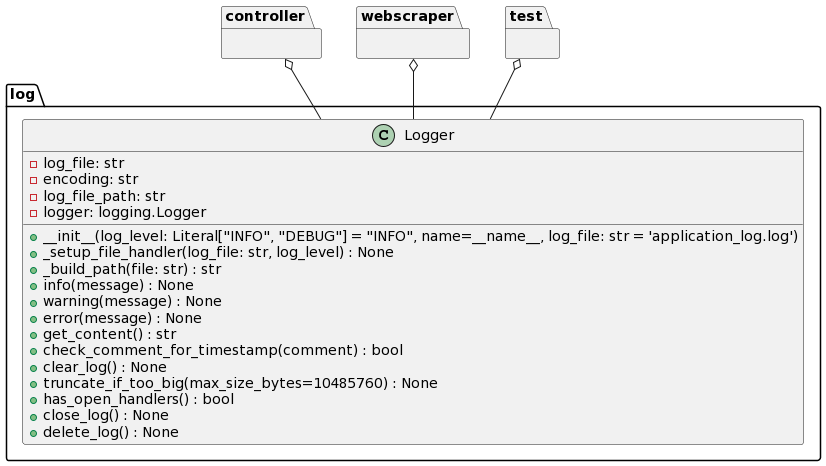
\includegraphics[width=0.8\linewidth]{img/class/logger}
	\caption{Logger UML Class Diagram}
	\label{img-logger-class}
\end{figure}

By default \emph{Logger} instances receive a log level of INFO and are referred to the \emph{application\_log.log}, however parameters exist to alter these settings upon initialization. 

Instances complete the initialization process by ensuring the log size has not exceeded the allotted 10 MB threshold. Upon passing this benchmark, truncation is ensured with the next instantiation.

The service allows the application to log messages of varying severity levels through the use of the \emph{info}, \emph{warning}, and \emph{error} methods. Messages logged under the base log level are omitted from the log file. This functionality allows different components to access the log for different purposes, and allow better control of what gets logged during debugging, testing, or runtime.

The logger also supports advanced operations, useful during testing and debugging, such as retrieving log file contents, patterns checking log contents, and managing the file itself.


\section{\emph{simulation}} \label{sec-simulation}
The package is responsible for setting up and running the Monte Carlo simulation, returning its findings for the parameterized epochs to the \emph{controller} package's host service. The package consists of four classes: \emph{GameBuilder}, \emph{Simulation}, \emph{MonteCarlo}, and the \emph{GameTools} static utility class.

The package's simulation constructor classes, the \emph{GameBuilder} and \emph{Simulation} classes, both utilize the static utility methods the \emph{GameTools} class in their logic. The enum service provided by the \emph{model} package is also used throughout the \emph{simulator} package, as depicted in Figure \ref{img-simulator-class} displaying the \emph{simulator}'s class diagram.

\begin{figure}[th!]
	\centering
	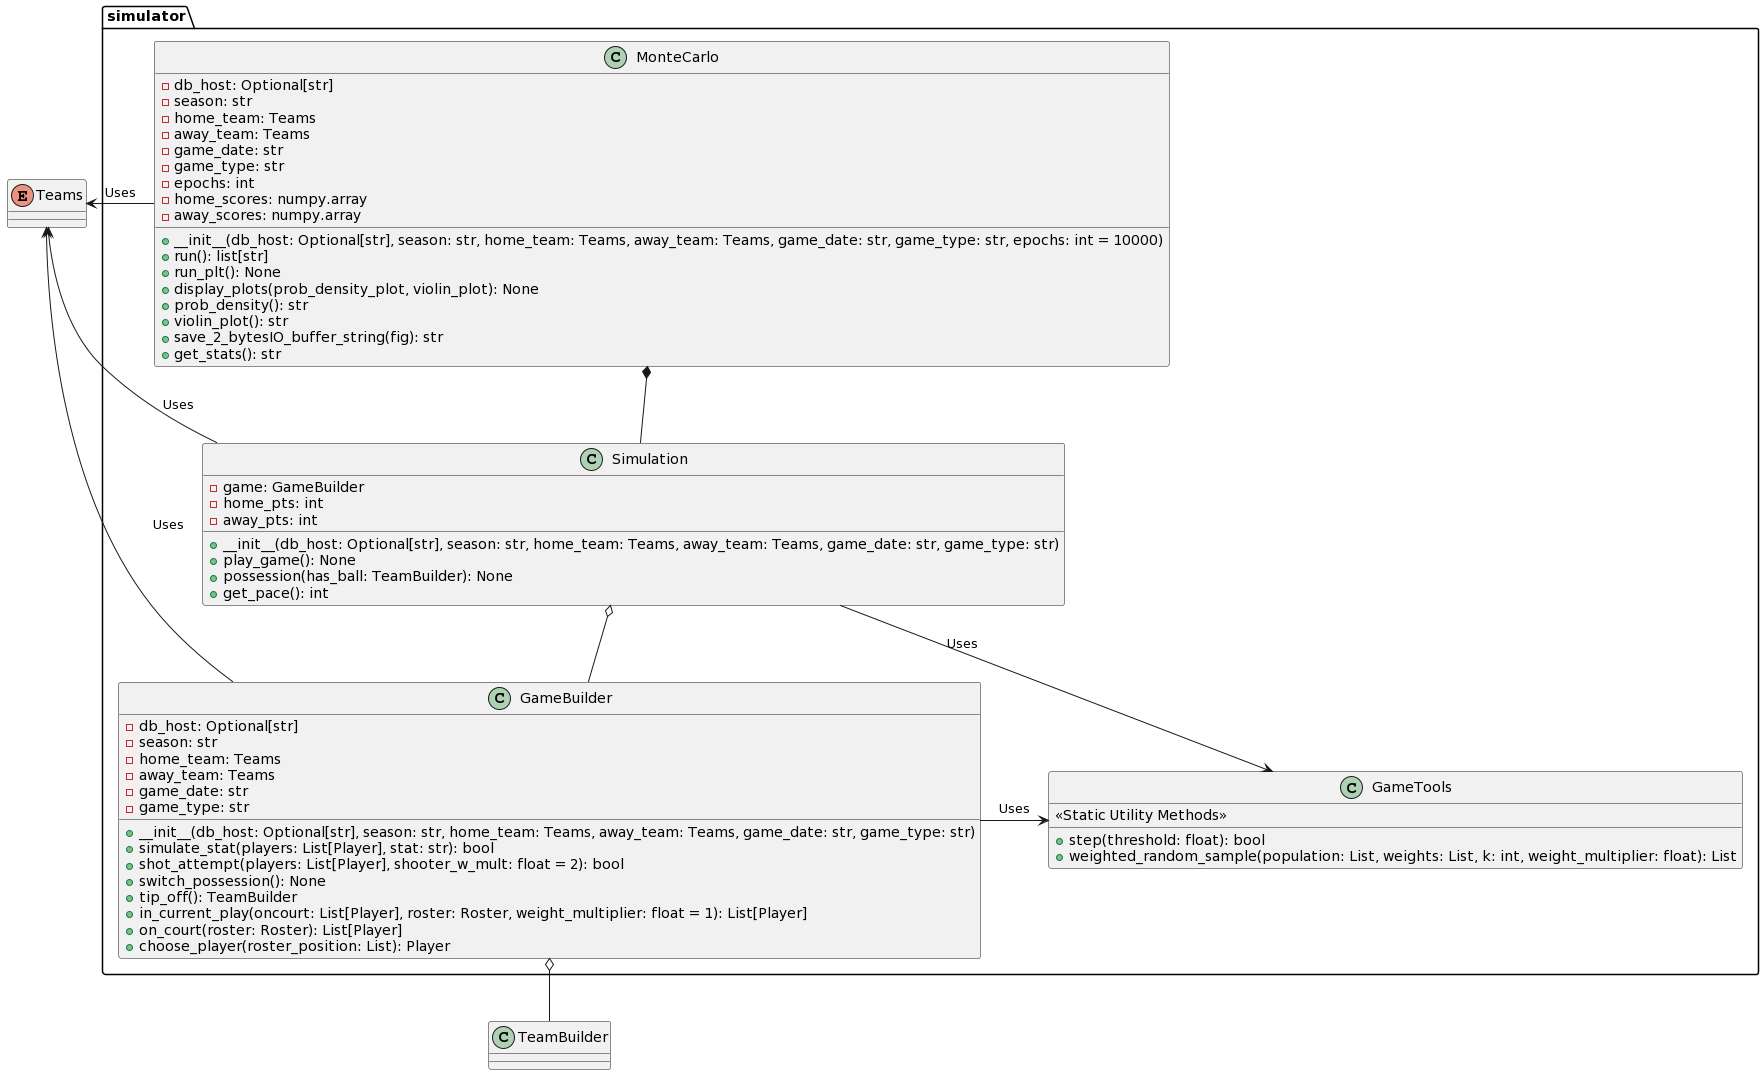
\includegraphics[width=1\linewidth]{img/class/simulator}
	\caption{\emph{simulator} UML Class Diagram}
	\label{img-simulator-class}
\end{figure}

\subsection{\emph{GameTools}}
The class contains static methods that provide non-deterministic results for the simulation process. This is done by introducing randomness through thresholds and weights in decision making. These methods are static for convenience upon use.

\paragraph{The Step Method:} This method makes decisions based on one parameterized metric, returning a boolean value of success or failure. A random float is generated between 0 and 1, and if it does not exceed the threshold (which is a float with the same boundaries) then the method returns a successful attempt. The threshold is utilized as an upper boundary, because higher statistical averages would otherwise lead to a smaller chance of success, requiring the negation of the results. Code Extract \ref{code-step} illustrates the method.
\lstinputlisting[caption=Step Method, label=code-step]{code/step.pas}

\paragraph{Player Sampling:} This method randomly selects players from a parameterized pool of options, applying weights to the decision making process. The effect of the weights on the selection process can be increased through the weight multiplier (which exponentiates the value) parameter. The required sample size is represented by k. Code Extract \ref{code-rand-sample} illustrates the method.
\lstinputlisting[caption=Weighted Random Player Sampoling Method, label=code-rand-sample]{code/rand-sample.pas}


\subsection{\emph{GameBuilder}}
The class utilizes \emph{TeamBuilder} instances to create the home and away teams parameterized during initialization. Its methods are focused on performing game related interactions, which assist the \emph{Simulation} class in completing the Monte Carlo simulation. 

Proceeding in chronological order relating to game-flow, the \emph{tip\_off} method simulates a tip off, deciding which team gets to attack first. The method selects the strongest rebounder (the player with the highest amount of offensive and defensive rebounds) from each team, then adds a home-court advantage of half the rebound delta between the home and away player's score. It then utilizes the \emph{GameTools}' step method to determine if the home team won the tip off. The team instance with possession of the ball is returned, and starts the flow of the game by filling the \emph{has\_ball} attribute.

Each possession randomly samples the players on the court, however not all players on the court participate in active game-play at all times. Therefore, the players on court are once again randomly sampled to decide which of them will actively participate in that single possession. The player sampling method is utilized to make these random selections. Each player's playtime\_w attribute serves as their respective weight in determining their likelihood of court time and active play time once on court. A combination of the \emph{on\_court}, \emph{choose\_player}, and \emph{in\_current\_play} methods provide this functionality.

The \emph{simualte\_stat} and \emph{shot\_attempt} methods randomly decide if their respective events come to pass by utilizing the step method. The first is meant to simulate metrics such as turn overs (when a player looses the ball for any reason), among other, and allows for further development of the simulation through its utilization on additional metrics to improve results. 

The \emph{shot\_attempt} method is specifically meant to deal with scoring attempts. It first decides who, of the players actively participating in the play will attempt to score the point. Then their shot metrics are reviewed to decide what type of shot they will attempt (3 point or regular 2 point). Code Extract \ref{shot-attempt} shows the method.
\lstinputlisting[caption=Weighted Random Player Sampoling Method, label=code-shot-attempt]{code/shot-attempt.pas}

Finally, the \emph{switch\_possession} method awards the ball to the opposing team, allowing them an offensive attempt in turn. Further functionality is added to the simulation through the utilization of these methods by the \emph{Simulation} class.


\subsection{\emph{Simulation}}
The class constructs a simulation instance which will play a single basketball game. The parameters and data reconstruct a specific historical match. Upon initialization, the class utilizes the \emph{GameBuilder} class to construct the game scenario, before proceeding with the simulation and returning the final score.

The pace\footnote{In a basketball game, the pace metric indicates the average or expected amount of possessions the team will have during the expected 48 minutes of play \cite{pace}.} of the game is determined by the combination of each teams relevant metric, providing the required number of possession iterations to conclude the match.

\textbf{The \emph{possession} method} applies the relevant logic encapsulated by the \emph{GameBuilder} instance to the parameterized \emph{TeamBuilder} object. After deciding which players are on court, and which of these are actively involved in play, the possibility of a turnover is reviewed. If the ball is turned over, the opposing team continues with their possession, otherwise a shot attempt is made. If the shot is unsuccessful, the rebound metrics are simulated to determine if the offensive team will attack again (this does not count as a new possession in the iteration), otherwise the ball is turned over to the opposing team. 

After the allotted number of iterations have concluded, the simulation can present the home and away scores representing the outcome of the single match.

\subsection{\emph{MonteCarlo}}
Monte Carlo simulation instances are initialized with parameters specifying a database connection, relevant game data, which then populates the necessary attributes required for operations, and the desired number of epochs.

The class provides two separate run methods, allowing for both client and back-end utilization. Client-based use is constructed specifically for the purpose of presenting this project for academic review, and is therefore limited by a connection time which consequently limits the amount of epochs. Back-end use is meant for higher epoch counts, placing less demand on the system. This is utilized to test the application's results with higher epoch counts, and determine how realistic the outcomes are.

Both methods create a \emph{Simulation} instance utilized to play one basketball game per epoch iteration. Results are tracked and returned as matplotlib plots, one probability density, and one violin. The back-end method \emph{run\_plt} displays the plots upon completion of the simulation, while the \emph{run} method, intended for client use, returns a list of the plots as strings, along with the basic statistics of the simulation such as the team's win percentage per the total number of epochs and the mode of their results. Code Extract \ref{code-convert} illustrates how the method utilized to convert matplotlib graphs to base64.

\lstinputlisting[caption=Plot Conversion to Base64, label=code-convert]{code/convert.pas}

\section{\emph{view}}
The package is a WinForms .NET framework application, and it acts as the client side of the system. Users can utilize the Windows-based program to communicate with the back-end's Python host via REST API. C\#'s RestSharp package provides the capability to handle HTTP requests and deserialize the returning responses into the appropriate objects for utilization.

The view is comprised of three windows: \emph{FindGame}, \emph{ScrapePopUp}, and \emph{MonteCarlo}. Each of these handles the communication necessary for their operation. The client operates only as a display, and an interface for the user. All operations are performed by back-end logic, and the results sent to the client as a JSON. Parameters are cached on the client side, decreasing the necessity of taking the same input parameters from the user. This information is also passed on to subsequent windows allowing for a smoother user experience.

The client only allows for simple, minimal client control of the application. Database operations are purposely limited to the back-end logic. The \emph{view} is truly a minimalist use interface intended to display the application's capabilities for the sake of presenting this project.

The \emph{FindGame} window takes initial parameters for setting up the game, such as home and away teams, season, and epoch count. When the \emph{Get Games} button is pressed, it requests all historic games via the \emph{/monte\_carlo/game\_data} resource endpoint, displaying them in a table via DataGridView \cite{dgv}.

The selected row automatically parameterizes the \emph{/monte\_carlo/team\_in\_db} endpoint, which notifies the client of the required data's presence, or lack thereof, in the database. If required, the \emph{ScrapePopUp} window appears, allowing the user to specify their choice of scrape settings to acquire the data with the \emph{/monte\_carlo/season\_data} endpoint. 

If the user wishes, web scraping can be forced, even if the data already exists by pressing the \emph{Forced Scrape} button. In this case all data is scraped again, however as all tables in the database require unique records, the data will only be added to the database if it is truly missing from a table.

The application does not include a VPN, therefore users are encouraged to use a third party service. Proxies are included with the application, and if turned on can provide an additional layer of security, however these are free proxy addresses that have not been thoroughly reviewed. They therefore cannot guarantee anonymity. Furthermore, the use of the built in proxies greatly decreases application speed, as the system will likely need a long time to locate one that is operational, due to the high demand for these services. Users do have the option to provide their own proxy list. If they choose to do so, they must provide it as a CSV table, with the first row being header, first column containing IP addresses, and second row containing port numbers.

Once it is established that the database contains the necessary information (either by means of a successful scrape, or by confirmation from the host), the final window is activated. This \emph{MonteCarlo} window receives all previous parameters from the previous windows upon initialization, and commences the simulation without the need for user interaction via the \emph{/monte\_carlo/simulation} endpoint, displaying both graphs along with original and simulated game data for the user.

Message boxes notify the user of any potential errors throughout the application process, giving brief descriptions. All errors are logged on the server-side of the application allowing for further debugging.


\section{\emph{webscraper}} \label{sec-webscraper}
The \emph{webscraper} package provides a variety of web scraping services, which are utilized and operated by the \emph{controller}. It provides both data acquisition and data parsing services through its \emph{ScraperFacade} and \emph{RealGMParser} classes. The facade class connects either directly or transitively to all other classes in the package. The \emph{RealGMParser} and \emph{ProxyHandler} class also make use of the \emph{Logger}. Figure \ref{img-webscraper-class} illustrates the package's class diagram.

This section reviews the \emph{webscraper}'s implementation broken down by functionality in order to give an overview of how they work together with the facade class that represents the package's functionality.

\subsection{Utility Classes}
The \emph{WebKit} class is a collection of static methods that are generally used by scrape services throughout the package. They attempt to mimic human use and introduce randomness to decrease the chance of being blocked by the service provider. Services include:
\begin{itemize}
	\item Creating new random headers for HTTP requests, mimicking varying operating systems and browser technologies.
	
	\item Introducing random with preset intervals for delays between requests.
	
	\item In case of Selenium utilization, providing mouse movements to specific elements within the HTML.
\end{itemize}

The \emph{ProxyHandler} class creates and returns a list of proxies, with the added capability to check each proxy before appending them to the list. While this functionality can be useful, it doesn't necessarily guarantee access to the proxy upon later use, as free proxies have a high demand online. The class also provides a default proxy list, however parameterization allows for the use of one's own list. Proxy lists must be CSVs, with the first row being the header, first column the IP addresses, and second the port numbers.

The \emph{ProxyKit} offers proxy services to chosen web scraping methodologies in the facade through it's proxy list attribute. The class contains methods to check proxy and IP address formats, and package them for utilization by the scraping methods (e.g.: Requests library's request method requires a dictionary format specifying the string separately for HTTP and HTTPS). The class also houses the \emph{apply\_rotating\_proxy} method, responsible for applying single proxies to the web scraping process. Each scrape attempt is assigned a new proxy. Addresses are popped from the list and attempt a connection. This process continues until a successful connection is made, after which the working proxy address is appended to the back of the list for future use.

\subsection{Selenium WebDrivers}
The Selenium service uses an abstract WebDriver acting as a base class, defining common virtual and regular methods for all implementing child classes. Each child class operates a separate browser technology, offering the same functionality. Methods pertaining to WebDriver setup are virtual, allowing each WebDriver instance to implement its browser specific setup options, providing, among other things, proxy functionality for later use. Regular methods provide web scraping capabilities and quit the driver.

The \emph{WebDriverFactory} is a factory class with static methods responsible for creating instances of the sub-classes, such as FirefoxDrivers and ChromeDrivers. This method is based on the Factory Method described in the GOF book Head First Design Patterns \cite[p.~134]{GOF}, and Abstract Factory Pattern \cite[p.~156]{GOF} which allows utilizing systems to decide which sub-class they want to create. The static factory methods allow further decoupling, by allocating sub-class instantiation to a separate static factory instead of utilizing the WebDriver for this task.

The code contains the setup for Undetected ChromeDriver, however it is not implemented (it's commented out), as the library has caused several bugs during testing, including issues with the numpy library and failing to delete instances after use. The code segments remain in the project because they are an interesting addition that merit further study and testing.

\subsection{The Facade}
The \emph{ScraperFacade} utilizes the Facade Design Pattern from the GOF's Head First Design Patterns, wherein a complex component architecture provides a single class which encompasses the package's functionality, and is consequently able to act as an access point for all utilizing services within the application \cite[p.~264]{GOF}. 

The facade therefore provides full data acquisition services to the \emph{controller}. It accesses the factory method to create Selenium driver instances, or creates HTTP content requests with Python's Requests library. Services provided by the \emph{WebKit} are automatically included in both. It also provides the necessary access methods to utilize proxies during web scraping.

\subsection{Parsing Service}
The \emph{RealGMParser} is treated as a standalone component within the package. The class consists of static utility methods, built for parsing and handling content acquired form the RealGM website's URLs. The class makes use of the BeautifulSoup4 and Pandas Python libraries to parse the scraped data into DataFrames.

\begin{figure}[th!]
	\centering
	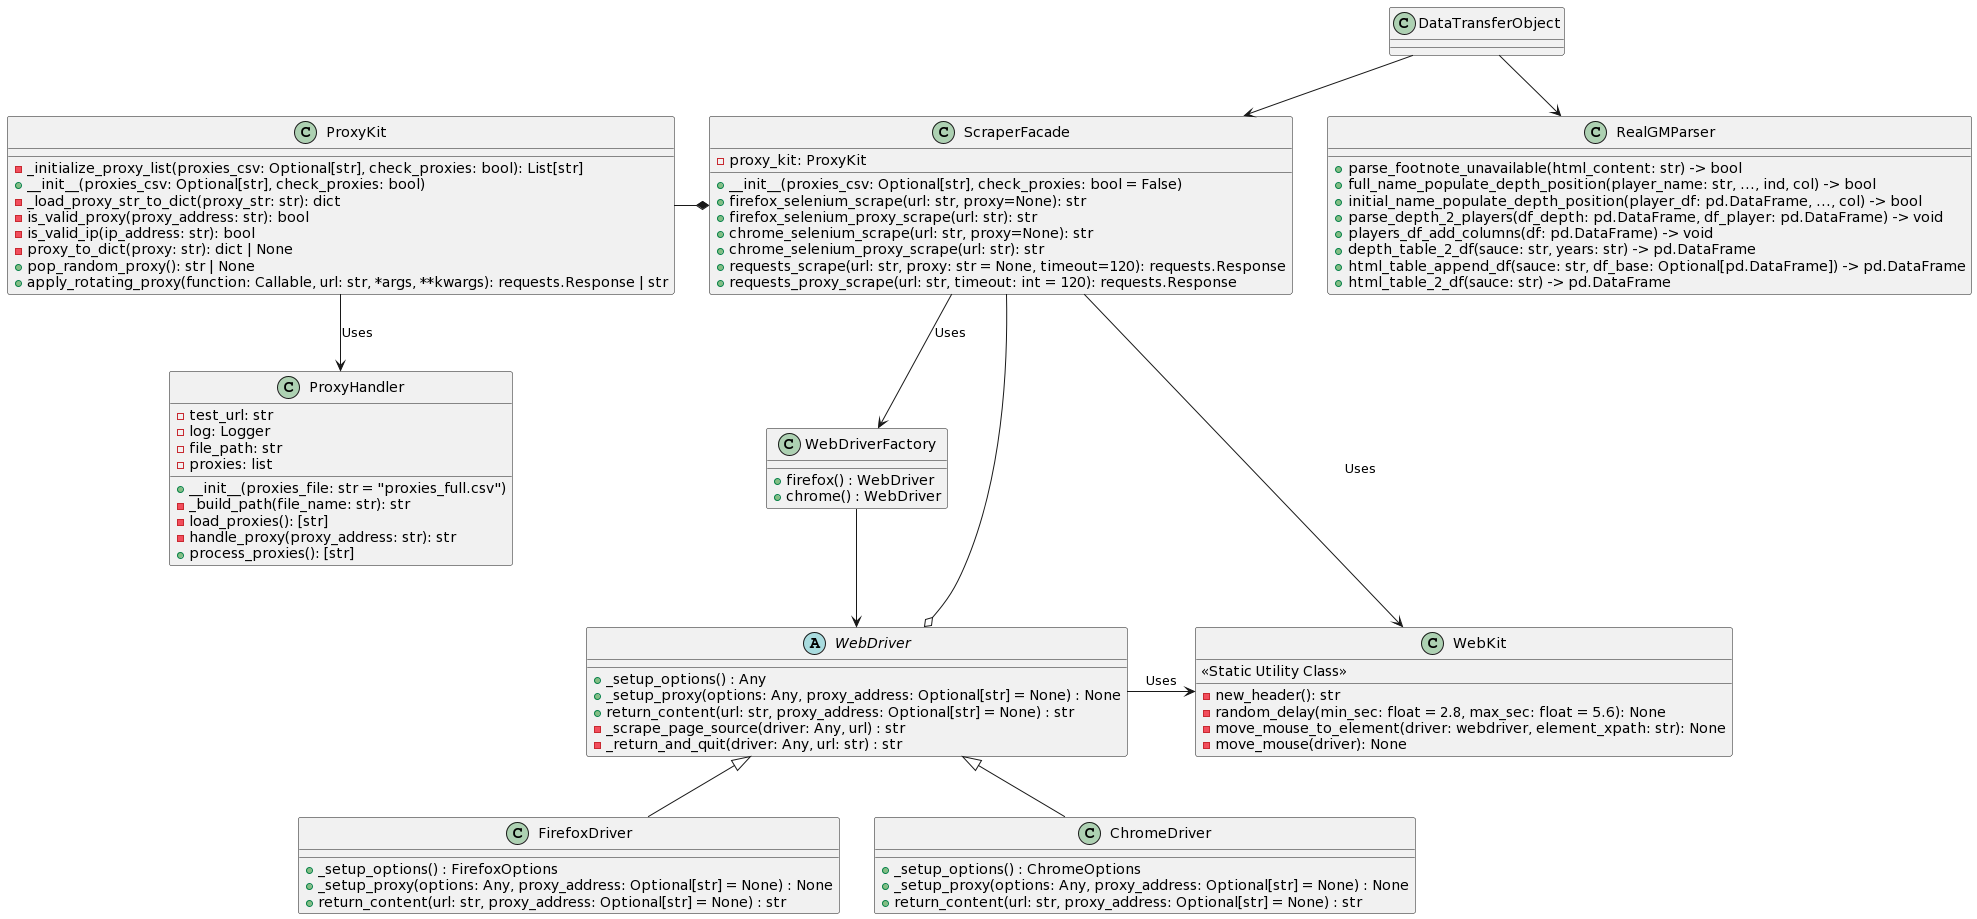
\includegraphics[width=1\linewidth]{img/class/webscraper}
	\caption{\emph{webscraper} UML Class Diagram}
	\label{img-webscraper-class}
\end{figure}


\chapter{Testing and Validation} \label{ch-testing}

\section{Unit Testing}
\section{Integration Testing}
\section{System Testing}
with white
\section{Performance Evaluation}

\chapter{Manual}
\section{Installation Guide}
\section{User Guide}

\chapter{Results and Discussion}
\section{Analysis of Web Scraping Results}
\section{Evaluation of Monte Carlo Simulations}
\section{Comparison with Existing Methods}
common to use scrapy. selenium is not preferred in general due to lack of speed. undetected chrome needs to be looked at further

\chapter{Conclusion}
\section{Summary of Findings}
\section{Contributions to Knowledge}
\section{Limitations and Future Work}





%SAMPLE----------------------------------------%


\begin{theorem}
Text.
\end{theorem}

\begin{proof}
Text.
\end{proof}

\begin{definition}
``Antinomies''
\end{definition}

\begin{remark}
Text.
\end{remark}
%END SAMPLE----------------------------------------%


\chapter{Appendices}

\section{Code Samples}
\section{GUI Mockups}
\section{Test Cases}


\begin{thebibliography}{2}
\addcontentsline{toc}{chapter}{\bibname}

\bibitem{Mondaut}
\textsc{Medium}, 
\emph {The Power of Data: Understanding Its Impact and Applications Across Various Domains}, Jonathan Mondaut, 2023, \url{https://medium.com/@jonathanmondaut/the-power-of-data-understanding-its-impact-and-applications-across-various-domains-6b3c2b2f1ca3}, [Retrieved 2 March 2024]

\bibitem{Kornwitz}
\textsc{Northeastern University, College of Science},
\emph{Why it’s so hard to make accurate predictions}, Jason Kornwitz, 2017, \url{https://cos.northeastern.edu/news/hard-make-accurate-predictions/}, [Retrieved 27 February 2024]

\bibitem{Khder}
\textsc{Moaiad Ahmad Khder},
\emph{Web Scraping or Web Crawling: State of Art, Techniques, Approaches and Application}, 
International Journal of Advance Soft Computing and Applications, 
Vol. 13, No. 3, 2021, 
Print ISSN: 2710-1274, Online ISSN: 2074-8523, 
Al-Zaytoonah University of Jordan

\bibitem{Aderibigbe}
\textsc{Adekitan Aderibigbe},
\emph{A Term Paper on Monte Carlo Analysis/Simulation},
Department of Electrical and Electronic Engineering,
Faculty of Technology, University of Ibadan,
2014.

\bibitem{NBA}
\textsc{Wikipedia},
\emph{National Basketball Association}, 2024, 
\url{https://en.wikipedia.org/wiki/National_Basketball_Association}, [Retrieved 27 February 2024]

\bibitem{McLeish}
\textsc{Don L. McLeish}: 
\emph{Monte Carlo Simulation and Finance}, 
Hoboken, New Jersey, USA, John Wiley \& Sons, Inc., 2005.

\bibitem{Steffen}
\textsc{Paul Steffen}:
\emph{Statistical Modeling of Event Probabilities Subject to Sports Bets: Theory and Applications to Soccer, Tennis, and Basketball},
Statistics [math.ST], Université de Bordeaux, 2022.
English.
NNT: 2022BORD0210.
tel-03891393.

\bibitem{Booch}
\textsc{Grady Booch, Robert A. Maksimchuk, Michael W. Engle, Bobbi J. Young, Jim Conallen, Kelli A. Houston},
\emph{Object-Oriented Analysis and Design with Applications}, 
Massachusetts, USA, Addison-Wesley, 2007.

\bibitem{Fowler}
\textsc{Martin Fowler, David Rice, Matthew Foemmel, Edward Hieatt, Robert Mee, Randy Stafford},
\emph{Patterns of Enterprise Application Architecture},
USA, Addison-Wesley Professional, 2002.

\bibitem{GOF}
\textsc{Eric Freeman, Elisabeth Freeman, Bert Bates, Kathy Sierra},
\emph{Head First Design Patterns},
O'Reilly, 2004.

\bibitem{GOF2}
\textsc{Spring Framework Guru},
\emph{National Basketball Association}, 2024, 
\url{https://springframework.guru/gang-of-four-design-patterns/}, [Retrieved 5 March 2024]

\bibitem{Kulliyyah}
\textsc{Abdul Rahman bin Ahlan, Murni bt Mahmud, Yusri bin Arshad},
\emph{Conceptual Architecture Design and Configuration of Thin Client System For Schools in Malaysia: A Pilot Project}, 
Department of Information System, Kulliyyah of Information and Communication Technology,
Kuala Lumpur, Malaysia, 2010.

\bibitem{Reade}
\textsc{Chris Reade},
\emph{Elements of Functional Programming}, 
Boston, USA, Addison-Wesley Longman, 1989.

\bibitem{Wiki-GUI}
\textsc{Wikipedia},
\emph{Graphical user interface}, 2024,
\url{https://en.wikipedia.org/wiki/Graphical_user_interface}, [Retrieved 5 March 2024]

\bibitem{enum}
\textsc{Microsoft Learn},
\emph{Enumeration types (C\# reference)}, Bill Wagner, 2023,
\url{https://learn.microsoft.com/en-us/dotnet/csharp/language-reference/builtin-types/enum} [Retrieved 6 March 2024]

\bibitem{mdn-html}
\textsc{MDN Web Docs},
\emph{HTML: HyperText Markup Language}, 2024,
\url{https://developer.mozilla.org/en-US/docs/Web/HTML}, [Retrieved 6 March 2024]

\bibitem{bs4}
\textsc{Beautiful Soup 4.12.0 documentation}, 
\emph{Beautiful Soup Documentation}, 2004-2023 Leonard Richardson,
\url{https://www.crummy.com/software/BeautifulSoup/bs4/doc/#}, [Retrieved 6 March 2024]

\bibitem{mdn-xml}
\textsc{MDN Web Docs}, 
\emph{XML: Extensible Markup Language}, 2024,
\url{https://developer.mozilla.org/en-US/docs/Web/XML}, [Retrieved 6 March 2024]

\bibitem{mdn-http}
\textsc{MDN Web Docs}, 
\emph{HTTP}, 2024
\url{https://developer.mozilla.org/en-US/docs/Web/HTTP}, [Retrieved 6 March 2024]

\bibitem{fake-useragent}
\textsc{PyPI Python Package Index},
\emph{fake-useragent}, 2023,
\url{https://pypi.org/project/fake-useragent/#description}, [Retrieved 6 March 2024]

\bibitem{req-head}
\textsc{MDN Web Docs}, 
\emph{HTTP headers}, 2024,
\url{https://developer.mozilla.org/en-US/docs/Web/HTTP/Headers}, [Retrieved 6 March 2024]

\bibitem{mdn-json}
\textsc{MDN Web Docs},
\emph{JSON}, 2024,
\url{https://developer.mozilla.org/en-US/docs/Glossary/JSON}, [Retrieved 7 March 2024]

\bibitem{wiki-http}
\textsc{Wikipedia},
\emph{HTTP}, 2024,
\url{https://en.wikipedia.org/wiki/HTTP}, [Retrieved 7 March 2024]

\bibitem{wiki-https}
\textsc{Wikipedia},
\emph{HTTPS}, 2024,
\url{https://en.wikipedia.org/wiki/HTTPS}, [Retrieved 7 March 2024]

\bibitem{flask}
\textsc{Pallets Projects},
\emph{Flask}, 
\url{https://flask.palletsprojects.com/en/3.0.x/}, [Retrieved 7 March 2024]

\bibitem{docs-flask}
\textsc{Read the Docs},
\emph{Flask}, 2024,
\url{https://readthedocs.org/projects/flask/}, [Retrieved 7 March 2024]

\bibitem{matplotlib}
\textsc{Matplotlib}, 
\emph{Matplotlib: Visualization with Python}, 2023,
\url{https://matplotlib.org/}, [Retrieved 7 March 2024]

\bibitem{wiki-mysql}
\textsc{Wikipedia},
\emph{MySQL}, 2024,
\url{https://en.wikipedia.org/wiki/MySQL}, [Retrieved 7 March 2024]

\bibitem{wiki-pd}
\textsc{Wikipedia},
\emph{pandas (software)}, 2024,
\url{https://en.wikipedia.org/wiki/Pandas_(software)}, [Retrieved 8 March 2024]

\bibitem{python}
\textsc{Python},
\emph{What is Python? Executive Summary},
\url{https://www.python.org/doc/essays/blurb/}, [Retrieved 8 March 2024]

\bibitem{req}
\textsc{Read the Docs},
\emph{Requests: HTTP for Humans},
\url{https://requests.readthedocs.io/en/latest/}, [Retrieved 8 March 2024]

\bibitem{restsharp}
\textsc{RestSharp},
\emph{Recommended usage}, Peter Breen, 2023,
\url{https://restsharp.dev/intro.html}, [Retrieved 8 March 2024]

\bibitem{redhat-rest}
\textsc{Red Hat},
\emph{What is a REST API?}, 2020, 
\url{https://www.redhat.com/en/topics/api/what-is-a-rest-api}, [Retrieved 8 March 2024]

\bibitem{selenium}
\textsc{Harvard Scholar},
\emph{Selenium Documentation Release 1.0}, 2012, 
\url{https://scholar.harvard.edu/files/tcheng2/files/selenium_documentation_0.pdf}, [Retrieved 8 March 2024]

\bibitem{udc}
\textsc{Github},
\emph{undetected-chromedriver}, 2024, 
\url{https://github.com/ultrafunkamsterdam/undetected-chromedriver}, [Retrieved 8 March 2024]

\bibitem{.net}
\textsc{Microsoft Learn},
\emph{Introduction to NET}, 2024, 
\url{https://learn.microsoft.com/en-us/dotnet/core/introduction}, [Retrieved 8 March 2024]

\bibitem{wiki-xampp}
\textsc{Wikipedia},
\emph{XAMPP}, 2024,
\url{https://en.wikipedia.org/wiki/XAMPP}, [Retrieved 8 March 2024]

\bibitem{docs-white}
\textsc{Read the Docs},
\emph{TestStack.White},
\url{https://teststackwhite.readthedocs.io/en/latest/}, [Retrieved 8 March 2024]

\bibitem{winforms}
\textsc{Microsoft Learn},
\emph{Desktop Guide (Windows Forms .NET)}, 2023,
\url{https://learn.microsoft.com/en-us/dotnet/desktop/winforms/overview/?view=netdesktop-8.0}, [Retrieved 8 March 2024]

\bibitem{mariaDB}
\textsc{MariaDB Foundation},
\emph{About MariaDB Server},
\url{https://mariadb.org/about/}, [Retrieved 9 March 2024]

\bibitem{agg}
\textsc{matplotlib},
\emph{The builtin backends},
\url{https://matplotlib.org/stable/users/explain/figure/backends.html}, [Retrieved 10 March 2024]

\bibitem{dto-wiki}
\textsc{Wikipedia},
\emph{Data transfer object}, 2024,
\url{https://en.wikipedia.org/wiki/Data_transfer_object}, [Retrieved 14 March 2024]

\bibitem{SDSU}
\textsc{San Diego State University Fowler College of Business},
\emph{What is an NBA Players True Offensive Value?}, 2020,
\url{https://business.sdsu.edu/news/2020/12/what-is-an-nba-players-true-offensive-value}, [Retrieved 15 March 2024]

\bibitem{mysql.conn}
\textsc{MySQL Developer Zone},
\emph{MySQL Connector/Python Developer Guide}, 2024,
\url{https://dev.mysql.com/doc/connector-python/en/}, [Retrieved 16 March 2024]

\bibitem{injection-attack}
\textsc{OWASP},
\emph{SQL Injection},
\url{https://owasp.org/www-community/attacks/SQL_Injection}, [Retrieved 17 March 2024]

\bibitem{pace}
\textsc{Basketball Reference},
\emph{Glossary},
\url{https://www.basketball-reference.com/about/glossary.html}, [Retrieved 18 March 2024]

\bibitem{dgv}
\textsc{Microsoft Learn},
\emph{DataGridView Class},
\url{https://learn.microsoft.com/en-us/dotnet/api/system.windows.forms.datagridview?view=windowsdesktop-8.0}, [Retrieved 18 March 2024]

\bibitem{Knuth}
\textsc{Donald Ervin Knuth}: 
\emph{Deformation modelling tracking animation and applications}, Berlin, Heidelberg, Springer, 2001.

\bibitem{Manning}
\textsc{Christopher Manning, Prabhakar Raghavan, Hinrich Sch\"{u}tze}: 
\emph{Introduction to Information Retrieval}, New York, USA, Cambridge University Press, 2008.
\end{thebibliography}

tools:
- draw.io
- plantuml.com
- chat.openai.com
- stackoverflow.com
- google scholar

ADD:
- installation

\end{document}